\documentclass[../main.tex]{subfiles}
\graphicspath{{\subfix{../UTIL/FIGS}}}
\begin{document}

\subsection{Stakeholder and Non-functional Requirements Definition} \label{derivation}
As described in section REF, the UCAV is needed to fulfil a number of roles for different stakeholders.
The primary stakeholders are: the operator; friendly parties; neutral parties; tactical commanders (TACOM); and interdisciplinary users (e.g.\ ground controllers).
Additionally, the customer as an organisation has needs that must be fulfilled.
These needs have been elicited as capabilities - what a stakeholder would ``walk up'' to the system to use it for.
They can also be seen as the reasoning behind the functional requirements.
In the axiomatic design methodology~\cite{Lee2006}, this corresponds to the \textit{Customer domain}.
The perspective of the operator and TACOM have been prioritised, with those of ground controllers, other parties, and the customer considered but to a lesser extent.
The capabilities heirarchy has been modelled in SysML using Enterprise Architect (see figure~\ref{fig:CapView}).

\begin{figure}[H]
    \centering
        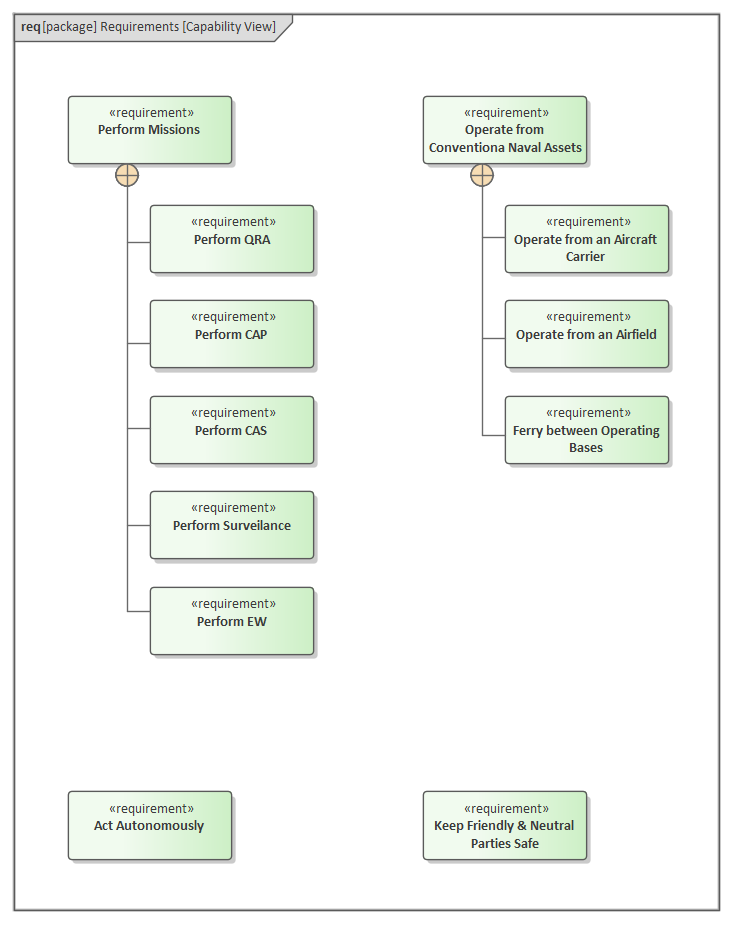
\includegraphics[width=.7\linewidth]{../UTIL/FIGS/Capability View.png}
        \caption[width=.7\linewidth]{UCAV Capability View}
        \label{fig:CapView}
\end{figure}

This simple view highlights the main missions that the UCAV will need to undertake:
\begin{itemize}
    \item Quick Reaction Alert (scrambling to interrogate a potential threat);
    \item Combat Air Patrol (loitering in an area to deter, detect, and defeat hostile targets);
    \item Close Air Support (striking ground targets near friendly land forces as directed by a controller);
    \item Surveilance (loitering or overflying an area to gather intelligence);
    \item Electronic Warfare (radiofrequency jamming).
\end{itemize}

It also captures some operational needs, key among which is operating from airfields or aircraft carriers.
Of secondary importance at this stage of the design is autonomous control, which is intimately connected with the safety of friendly and neutral parties.
As the design progresses and the wider system of systems is understood, these will likely into key capabilities that the UCAV must provide, and as such may be further decomposed.
One shortfall of the capability model is the lack of reference to some significant capabilities.
For example, cost would likely be a driving factor in the award of a contract by a customer so at this stage should be paramount.
The model does however provide a good starting point for functional requirement elicitation and clear justification for them, from an aerodynamic design standpoint.

From these capabilities, a set of functional and non functional requirements have been derived.
These are grouped into four on the diagram titled ``Requirements''.
The functional requirements under ``mission effectiveness'' were identified initially, and they are traceable back to the capabilities using \texttt{<<deriveReqt>>} relationships.
These relationships are hidden to improve readability of the diagram.
As is shown in figure~\ref{fig:ID3toID1}, a number of ``Aerial Performance'' requirements were then derived from these functions, with ``Operation and Support Functions'' and some other functional requirements in ``Aerial Performance'' being again derived from the capabilities.

\begin{figure}[H]
    \centering
        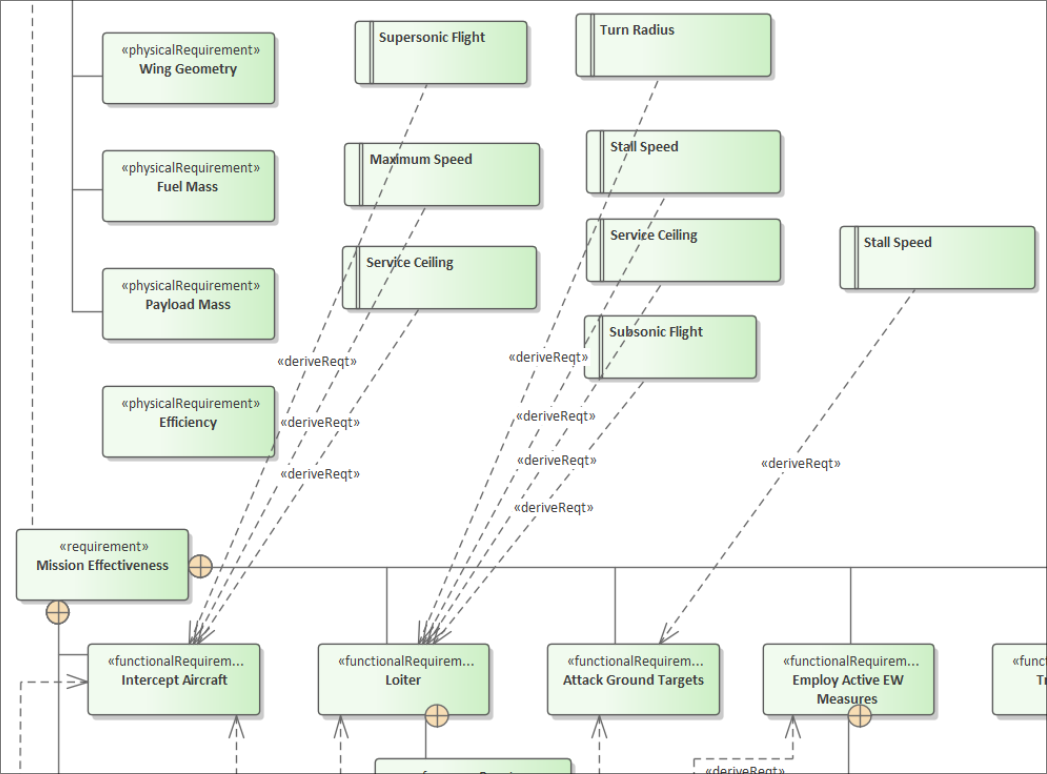
\includegraphics[width=.7\linewidth]{../UTIL/FIGS/id1-derive-id3.png}
        \caption[width=.7\linewidth]{Derivation of Aerial Performance requirements from Mission Effectiveness. Virtualised connector endings have been used for readability.}
        \label{fig:ID3toID1}
\end{figure}

In addition to functional requirements, some non-functional requirements have been derived.
From this paper's standpoint, a focus has been given to aerodynamic performance requirements, insofar as they enable the highest priority functions (see Section~\ref{reqrank}).
values for these performance requirements, where applicable, have been derived from contemporary fighter aircraft data (where it is publically available).
Table~\ref{tab:aircraft_parameters} contains information for five different aircraft~\cite{Roskam1989}: the F-4E Phantom II~\cite{F4-CD0}\cite{J72T}\cite{F4EAero}\cite{F-4EPerf}, the F15-C Eagle~\cite{F15-F18-CD0}\cite{F15CLmS}\cite{F15Thrust}, the F/A-18 Hornet~\cite{F15-F18-CD0}\cite{F18CLm}\cite{F18SAR}, the AV-8B Harrier~\cite{AV8BCLmax}\cite{AV8BTurnRate} (all McDonnel Douglas) and the Grumman A6-A intruder~\cite{A6A-AR}.
All are naval aircraft, aligning with the intended market of the UCAV\@.
This data has been used to inform engineering judgement on performance requirements, along with ``Physical Characteristics''.

\begin{table}[htbp]
    \centering
        \caption{Aircraft Performance and Aerodynamic Parameters}
    \label{tab:aircraft_parameters}
    \begin{tabular}{lccccc}
        \hline
        Parameter & F-4E & F-15C & F/A-18A & AV-8B & A-6 \\
        \hline
        $p_{s}$      & 0.356 & 0.334 & 0.357 & 0.219 & 0.330 \\
        $S \left[m^{2}\right]$       & 50.911 & 55.649 & 37.161 & 21.368 & 48.310 \\
        $C_{L\max}$ & 1.2 & 2.1 & 1.7 & 1.435 & 2.1 \\
        $m_{pl} \left[kg\right]$     & 1285 & 1451 & 3649 & 2314 & 907 \\
        $AR$      & 2.77 & 3.01 & 3.52 & 4 & 5 \\
        $T\left[N \times No.Engine\right]$       & $79620 \times 2$ & $106000 \times 2$ & $71000 \times 2$ & 105868 & $37000 \times 2$ \\
        $TSFC\left[\frac{kg}{Ns}\right]$    & $2.40\times10^{-5}$ & $2.07\times10^{-5}$ & N/A & $2.24\times10^{-5}$ & $2.32\times10^{-5}$ \\
        $m_f \left[kg\right]$     & 5469 & 6103 & 5503 & 3519 & 3975 \\
        $C_{D0}$  & 0.0205 & 0.0218 & 0.0239 & N/A & 0.023 \\
        $V_{\text{stall}} \left[ms^{-1}\right]$ & 52.4 & 39.4 & 60.1 & 62.5 & -- \\
        $ROC\left[ms^{-1}\right]$     & 294 & 390 & 152 & N/A & -- \\
        $R\left[m\right]$       & 1825 & 2193 & N/A & 807 & -- \\
        $r_{\text{Turn}}\left[m\right]$ & 280.6 & 158.5 & 368.3 & 397 & -- \\
        \hline
    \end{tabular}
\end{table}

\subsection{Requirements Analysis} \label{reqrank}
To determine which requirements were of highest priority, the analytic hierarchy process (AHP) was used.
Compared to other potential requirement ranking methods, AHP allows for an individual to determine the priorities from their specific standpoint on a case-by-case basis, which is something that other methods (e.g. \$100) do not allow. Additionally, as the majority of the requirements elicited use the terms ``must'' or ``shall,'' it is not possible to differentiate based on language (e.g. MoSCoW).
The input relationships can be seen in figure~\ref{fig:AHPInput}.
In each comparison, preference was given to requirements aligned with CAP to align with the intended market niche.
Autonomy was de-prioritised, as whilst it is an important facet of the UCAV, it has little impact on the airframe, propulsion and outfit.
The impacts it does have (e.g. no cockpit, no life support, turns no longer being human limited etc.) have not been considered to manage complexity and should be investigated in a follow up design study.

\begin{figure}[H]
    \centering
        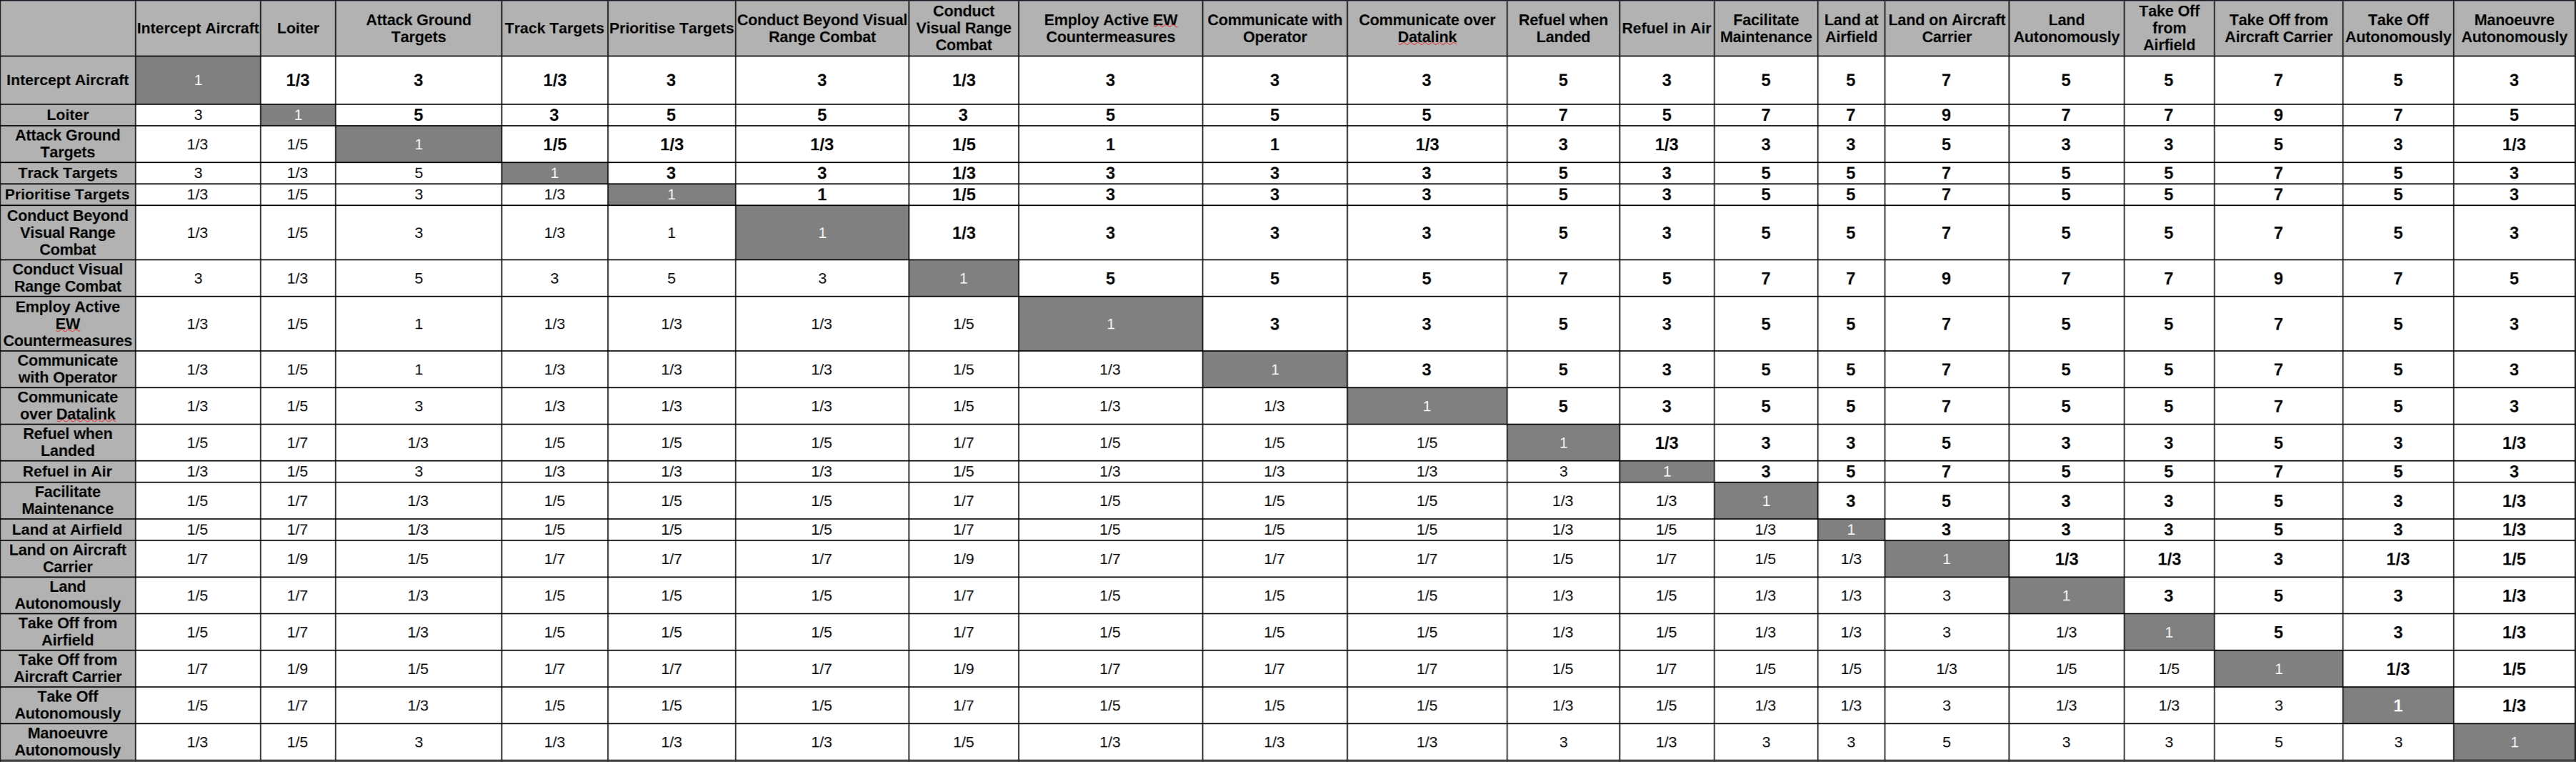
\includegraphics[width=\linewidth]{../UTIL/FIGS/AHP.png}
        \caption[width=.7\linewidth]{Requirement AHP matrix. As values are reciprocal below the diagonal, values above have been emphasised.}
        \label{fig:AHPInput}
\end{figure}

A python script was then used to calculate the normalised eigenvector for the respective requirements.
These eigenvectors can be seen in table~\ref{tab:ranked_requirements}.
From this, it is clear that the key requirements to focus on are loitering and within visual range combat. This is expected, as they are key components of CAP.
This was used as the base for non-functional derivation in Section~\ref{derivation}, but of note is that the derived requirements often apply to other functional requirements as well (such as Stall Speed relating to Attack Ground Targets).
This requirements ranking also indicates where future work can perform more complex design optimisations.

\begin{table}[htbp]
    \centering
        \begin{tabular}{r l r}
            \hline
            \textbf{Rank} & \textbf{Requirement} & \textbf{Weight} \\
            \hline
            1  & Loiter                              & 0.169 \\
            2  & Conduct Visual Range Combat         & 0.146 \\
            3  & Track Targets                       & 0.0980 \\
            4  & Intercept Aircraft                  & 0.0852 \\
            5  & Conduct Beyond Visual Range Combat  & 0.0698 \\
            6  & Prioritise Targets                  & 0.0690 \\
            7  & Employ Active EW Countermeasures    & 0.0574 \\
            8  & Communicate with Operator           & 0.0513 \\
            9  & Communicate over Datalink           & 0.0482 \\
            10 & Refuel in Air                       & 0.0400 \\
            11 & Manoeuvre Autonomously              & 0.0304 \\
            12 & Attack Ground Targets               & 0.0295 \\
            13 & Refuel when Landed                  & 0.0208 \\
            14 & Facilitate Maintenance              & 0.0186 \\
            15 & Land at Airfield                    & 0.0158 \\
            16 & Land Autonomously                   & 0.0141 \\
            17 & Take Off from Airfield              & 0.0126 \\
            18 & Take Off Autonomously               & 0.0108 \\
            19 & Land on Aircraft Carrier             & 0.00751 \\
            20 & Take Off from Aircraft Carrier      & 0.00649 \\
            \hline
        \end{tabular}
        \caption{Ranked requirements and their corresponding weights, to three significant figures.}
        \label{tab:ranked_requirements}
\end{table}

\subsection{Design Problems Definition and Specification}
From the derived and ranked requirements, a multi-objective optimisation problem was set up such that the optimal combination of the key design variables (DVs) can be found to optimise the design objecives (DOs).
The DOs are defined by the requirements; performance requirements set constraints on certain characteristics, and these characteristics are what should be optimised.
The DVs are values that the aircraft designer has control over.
Linking the two are design enablers (DEs), which are mathematical relationships that provide a value for a DO from a combination of DVs.
The combination of DVs, DEs, and DOs is termed a design problem.
The key performance requirements are stall speed $\left(V_{stall}\right)$, turn radius $\left(r_{turn}\right)$, range $\left(R\right)$, and rate of climb $\left(ROC\right)$.
These have been modelled using \texttt{<<constraint>>} blocks in SysML, as is seen within the Constraints boundary on the Requirements diagram (see figure~\ref{fig:DOConstraint}).

\begin{figure}[H]
    \centering
        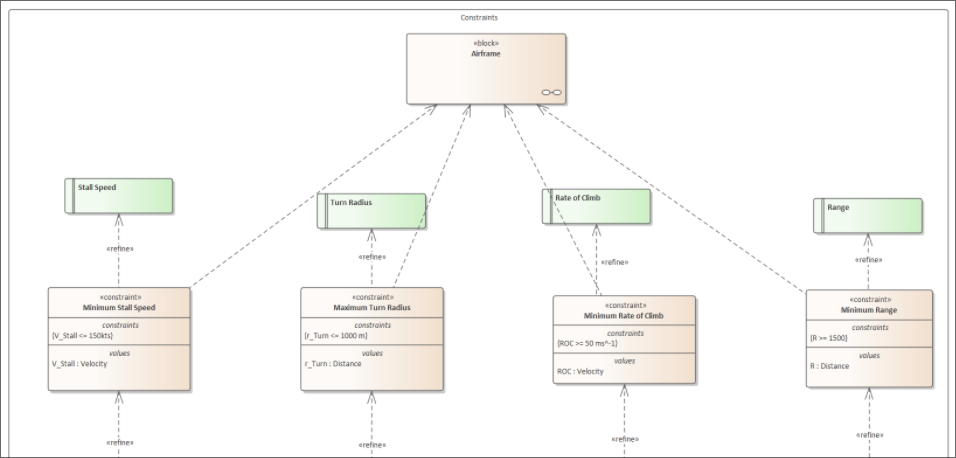
\includegraphics[width=.7\linewidth]{../UTIL/FIGS/DOconstraints.png}
        \caption[width=.7\linewidth]{DO constraint relationships to requirements and architecture}
        \label{fig:DOConstraint}
\end{figure}

These constraints are then refined by constraint blocks containing the DEs.
The DEs are based on classical aerodynamic equations.
Stall speed is derived from the well-known lift equation~\cite{VStall}:
\[
    L = \frac{1}{2}\rho V^{2} S C_{L}
\]

where $L$ is lift, $\rho$ is the density of air, $V$ the freestream speed, $S$ the wetted wing area, and $C_{L}$ the lift coefficient.
In steady flight, the aircraft is producing lift equal to its weight, such that it does not sink.
At stall, $V$ is set as low as it can be.
Therefore, as $\rho$ and $S$ do not change, $C_{L}$ must be maximised, and this limit is what defines the stall speed.
\begin{align*}
    W &= \frac{1}{2}\rho V_{stall}^{2} S C_{Lmax} \\
    \Rightarrow V_{stall} &= \left(\frac{2 W}{\rho S C_{Lmax}}\right)^{\frac{1}{2}}
\end{align*}

To determine turn radius a similar condition is used~\cite{minTurnAndLift}.
With the maximum wing loading $n_{max} \equiv \frac{L_{max}}{W}$,
\[
    r_{turn} = \frac{V^{2}}{g \left(n_{max}^{2} - 1\right)^{\frac{1}{2}}}
\]

Determining rate of climb also considers the thrust avaiable to the aircraft.
Specifically, it requires the excess thrust - the amound of thrust that exceeds the drag at a given freestream speed.
It is calculated using the following equation~\cite{ROC}:
\[
    ROC = \frac{\left(T - D\right)V}{W}
\]

where $T$ is the total thrust, $D$ the calculated drag, and $W$ the weight.
Drag can be calculated in the same manner as lift:
\[
    D = \frac{1}{2}\rho V^{2} S C_{D}
\]
$C_{Lmax}$ is a function of aircraft geometry, whereas $C_{D}$ is actually composed of multiple parts, however: the zero lift drag, and the lift-induced drag.
This can be represented with the \textit{drag polar}:
\[
    C_{D} = C_{D0} + \frac{C_{L}^{2}}{\pi e AR}
\]
where $C_{D0}$ is the zero lift drag coefficient (another geometric property), $AR$ the aspect ratio of the aircraft (a measure of a wing's ``slenderness''), and $e$ the Oswald efficiency factor.
$e$ is a measure of how closely a wing's lift distribution is to a purely elliptical distribution; for the purpose of this paper, a constant value of 0.8 is reasonable~\cite{oswald}.
Now, whilst $C_{Lmax}$ is a geometric property, $C_{L}$ is a function of the freestream velocity as the aircraft will only produce as much lift as is needed to counteract its weight.
\[
    C_{L} = \frac{2 W}{\rho S V^{2}}
\]

Finally, the range is calculated using the Breguet Range Equaiton~\cite{RangeEqn}:
\[
    R = \frac{V}{TSFC} \frac{CL}{CD} \ln\left(\frac{W_{i}}{W_{f}}\right)
\]
Where $W_{i}$ is the initial weight of the aircraf at take off (i.e.\ fuel, payload, and structure) and $W_{f}$ is the final weight (i.e. payload and structure, with all fuel burnt).
For this paper, all instances of $W$ have been $W_{i}$, and that can be calculated from the mass of the fuel $m_{f}$, mass of payload $m_{pl}$, acceleration due to gravity $g\equiv 9.81$ and proportion of the aircraft's overall weight which is structure $p_{s}$ (from~\cite{Roskam1989}):
\[
    W = \frac{g(m_{f} + m_{p})}{1 - p_{s}}
\]

TSFC is the thrust specific fuel consumption, and is a measure of the fuel used to produce a unit thrust.
It is normally published by the engine manufacturer or identified in reports (see table~\ref{tab:aircraft_parameters})

To represent these in SysML, constraint blocks were again used with the equations as constraints, and the DVs as values.
To do this, however, the DVs must exist somewhere in the model. 
A simple physical architecture was generated in the ``Architecture'' diagram.
This architecture is composed of four subsystems, with the key subsystem being the airframe (as all of the DOs are in some way aerodynamic metrics).
These subsystems are decomposed into lower level parts, which at this point are present for representation.
The airframe subsystem then contains value properties, which correspond to the performance metrics (DOs) but also the DVs.
Other values related to other subsystems (e.g. $m_{f}$) were assigned to their respective blocks, and ports permit the transfer of this information to the airframe block.
This is so that they can appear in parametric diagrams, which are owned by the airframe block.
Each DV is given bounds with constraint blocks, based on the data in table~\ref{tab:aircraft_parameters}.
Each DO has a corresponding parametric diagram, which shows diagramatically the flow of DVs through to the constraints set by the performance requirements, enabling traceability throughout the model.
The diagrams are titled Range, Rate of Climb, Stall Speed, and Turn Radius. An example is shown in figure~\ref{fig:StallSpeedPara}

\begin{figure}[H]
    \centering
        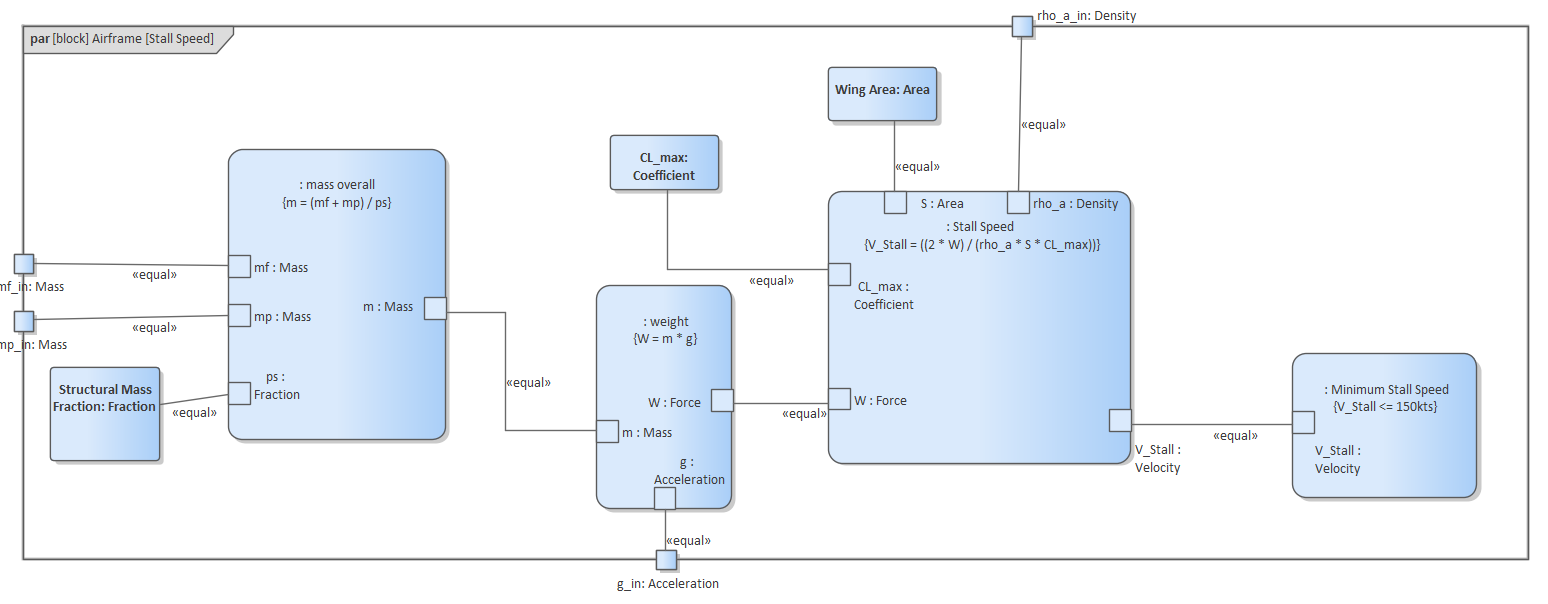
\includegraphics[width=\linewidth]{../UTIL/FIGS/Stall Speed.png}
        \caption[width=.7\linewidth]{Stall Speed Parametric Diagram}
        \label{fig:StallSpeedPara}
\end{figure}

\subsection{Design Analysis Plan and Methodology}
For analysis and visualisation, these DEs were coded in the Python programming language.
Python has many modules which allow for scientific computation and visualisation, namely numpy, pandas, and matplotlib.
These tools were used to display a matrix of scatter plots, showing pairwise relation between DVs and DVs, DVs and DOs, and DOs and DOs.
To generate the points, the module pydoe was used to implement Latin Hypercube Sampling, taking a number of points between the bounds and finding the corresponding DO values.
Additionally, scikit-learn allows for machine learning algorithms to be used.
In this case, it was used to perform ordinary least squares regression to provide partial dependency plots, which are plots essenstially showing the sensitivity of the DOs to each DV, mapping a response surface.

Figures~\ref{fig:SM1} and~\ref{fig:RStool} show this visualisation.

\begin{figure}[H]
    \centering
        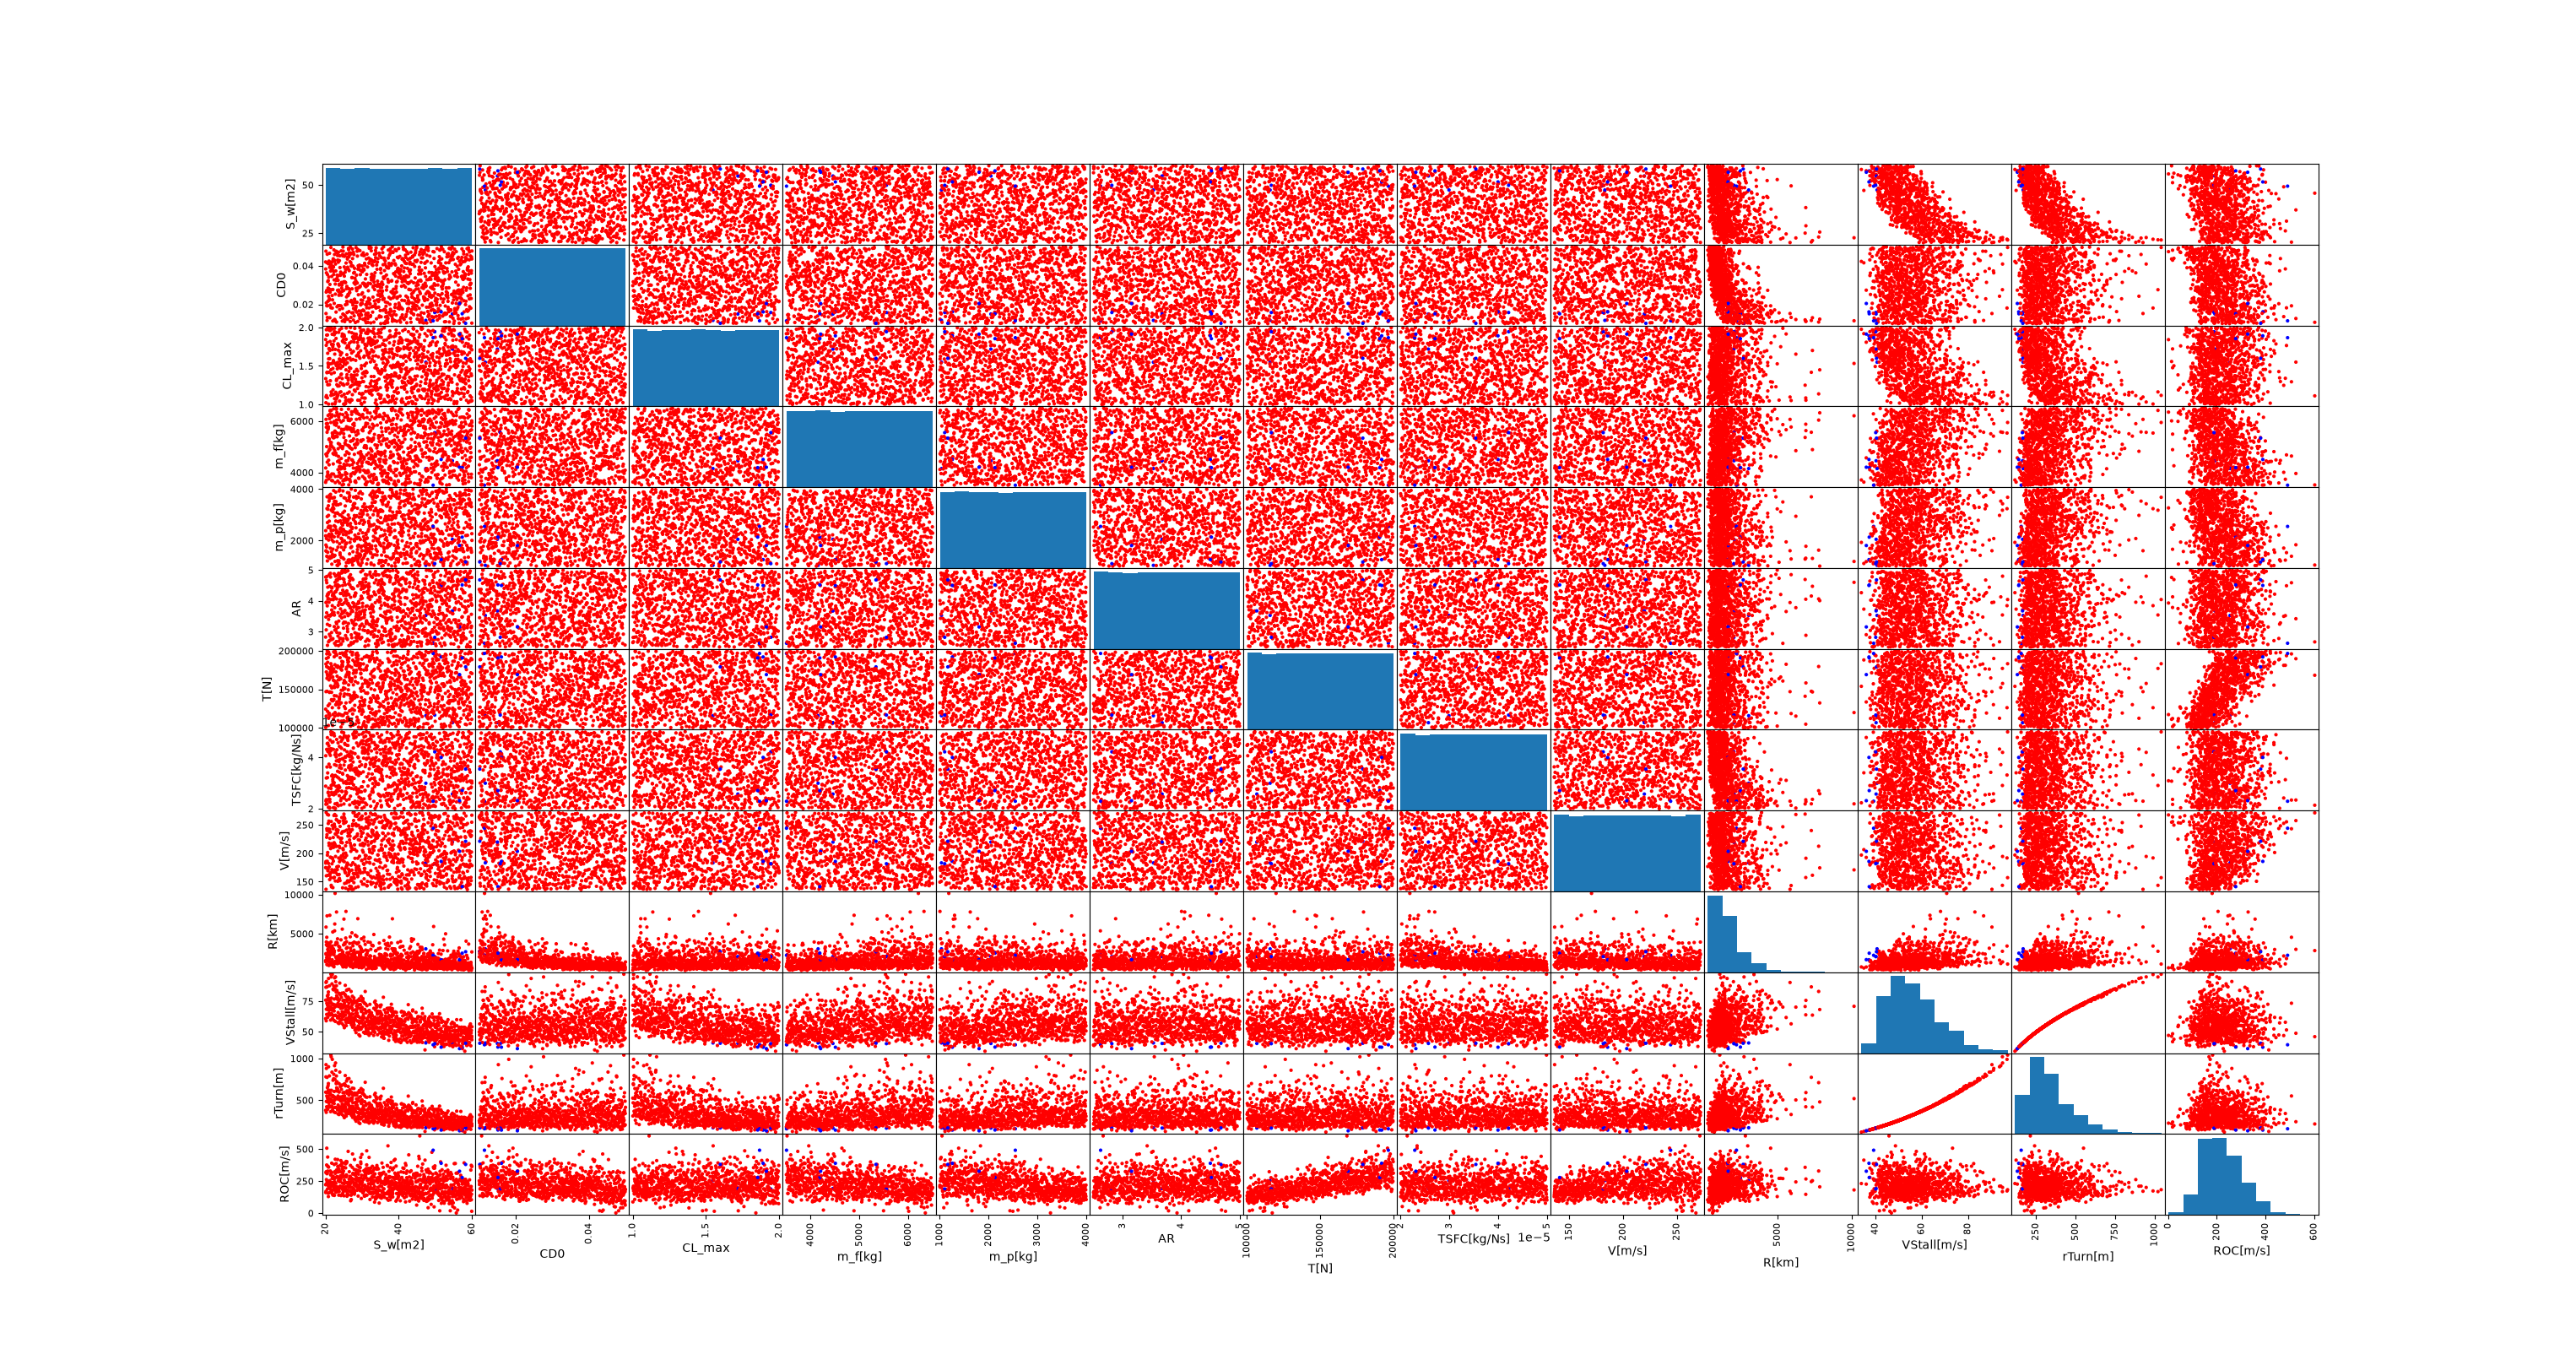
\includegraphics[width=\linewidth]{../UTIL/FIGS/multiple-scatter-matrix.png}
        \caption[width=.7\linewidth]{Initial design space visualisation}
        \label{fig:SM1}
\end{figure}

\begin{figure}[H]
    \centering
        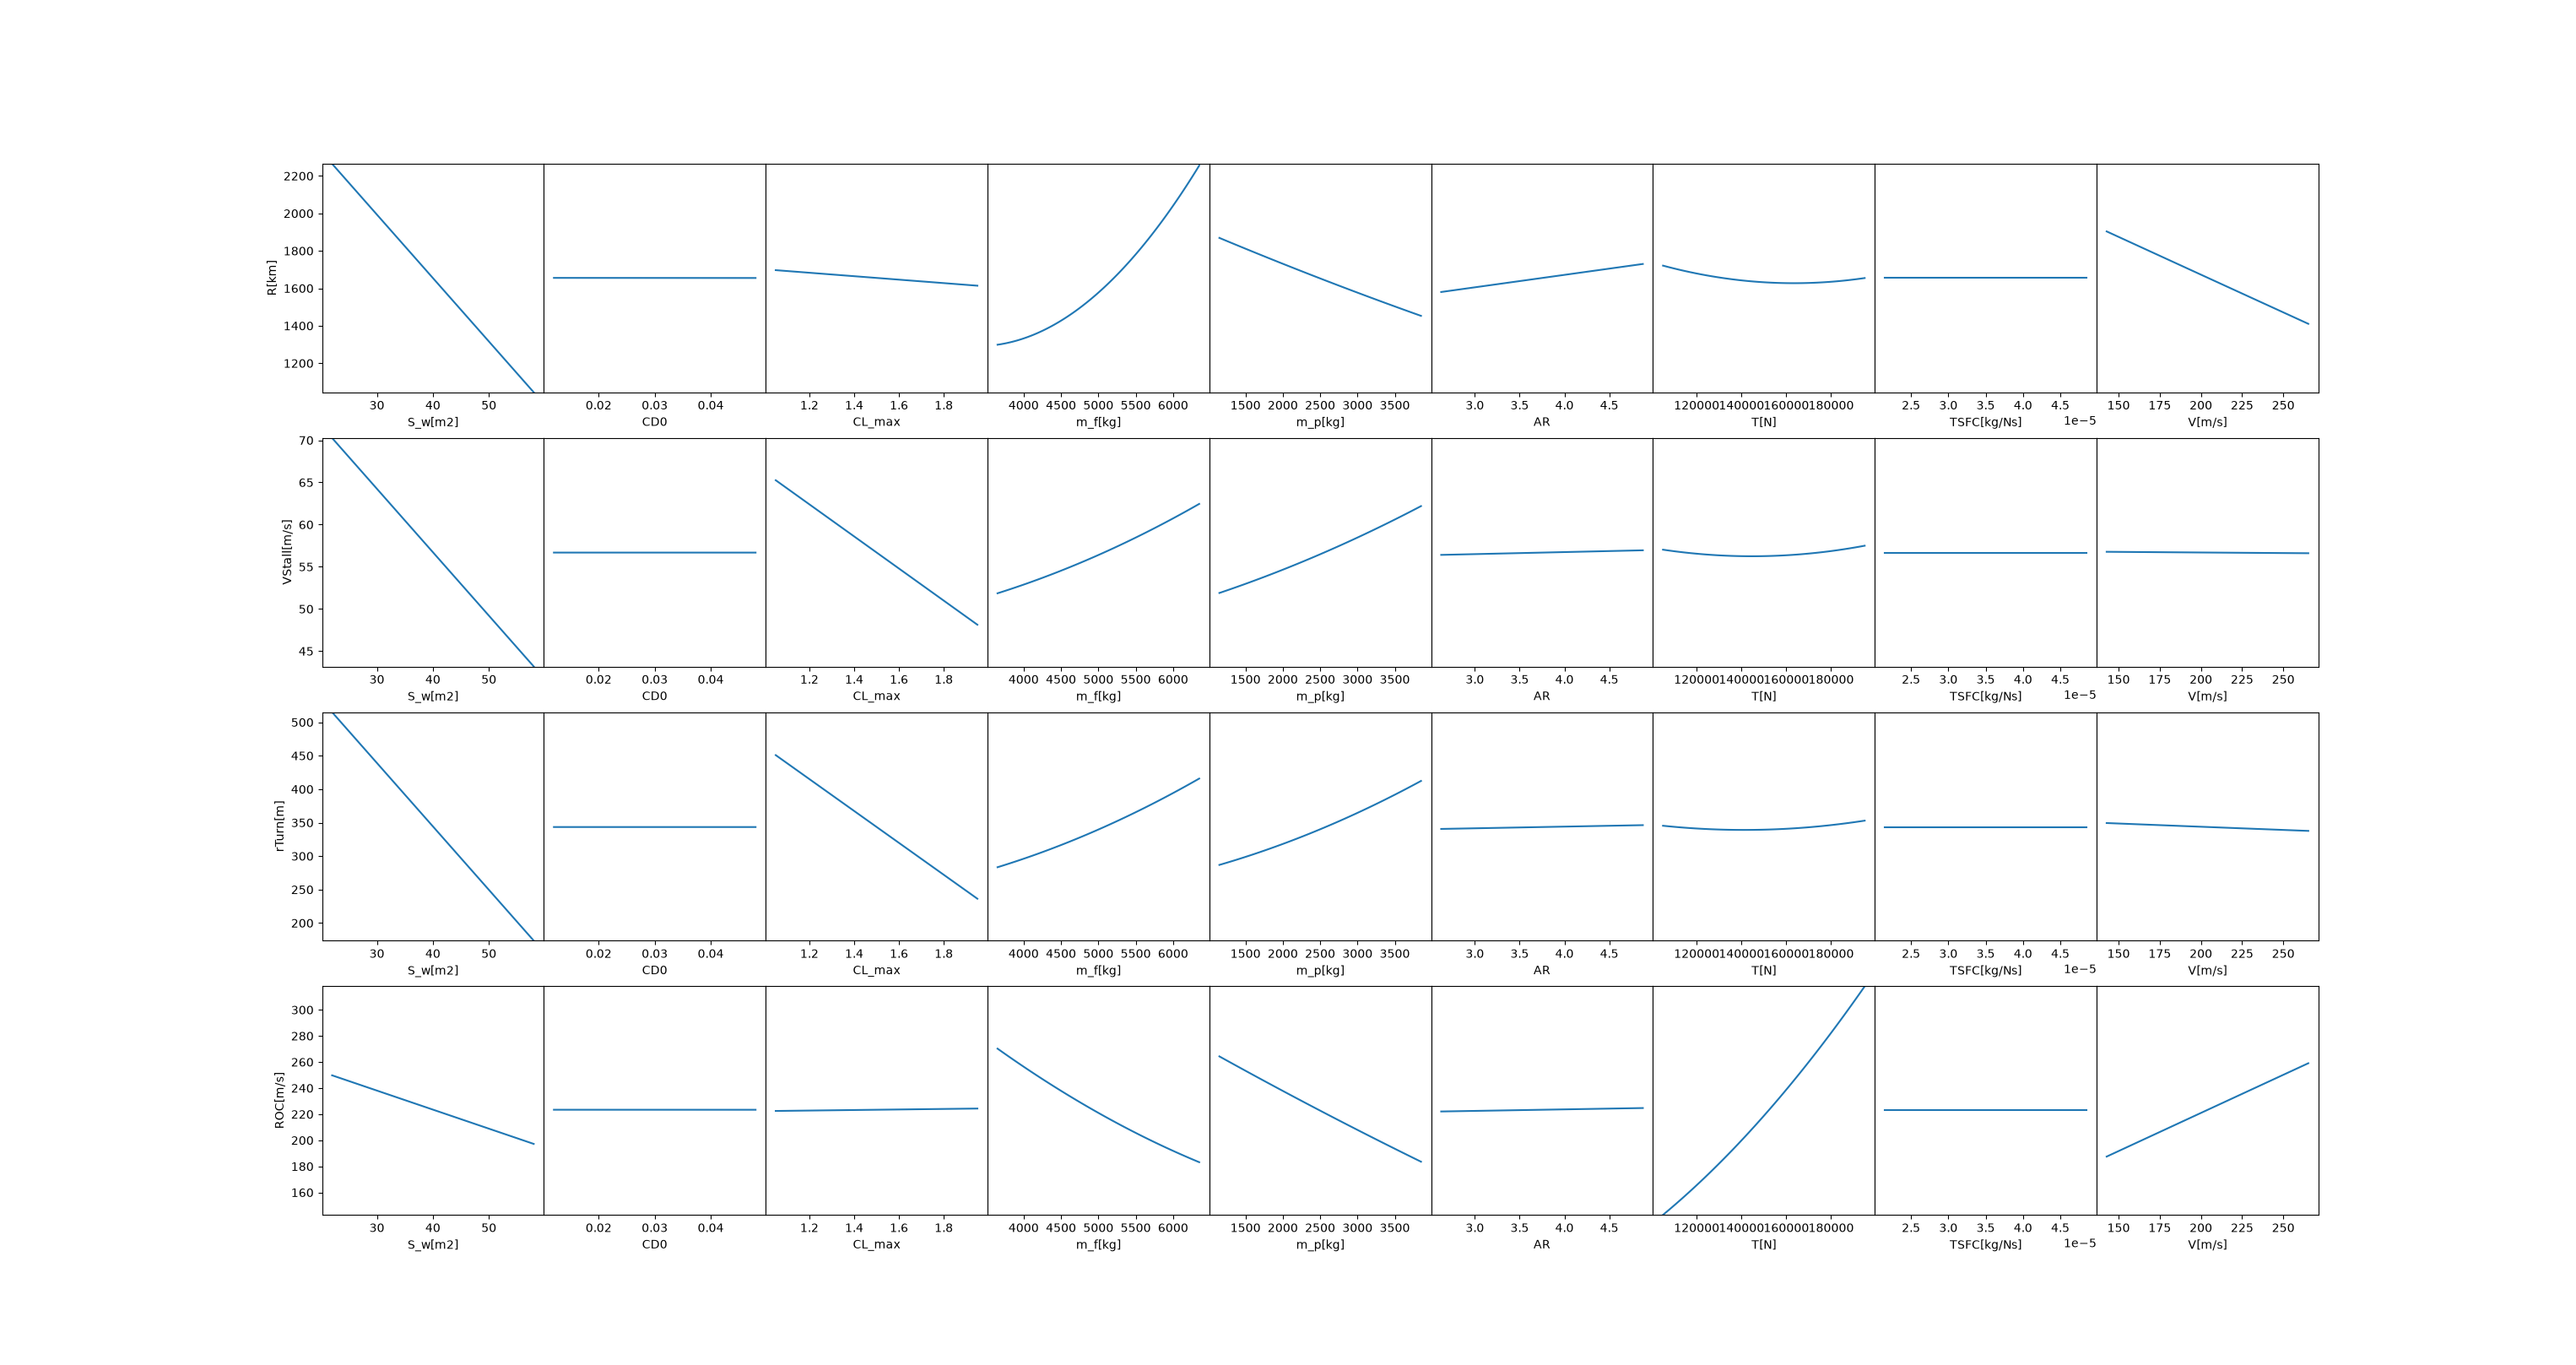
\includegraphics[width=\linewidth]{../UTIL/FIGS/multiple-rstool.png}
        \caption[width=.7\linewidth]{Sensitivity analysis of the design space}
        \label{fig:RStool}
\end{figure}

Attempting to optimise all 9 DVs simulatenously would be computationally expensive and potentially impossible.
Instead, fixing certain DVs and optimising the remaining ones individually is simpler and more likely to produce a suitable result.
In the axiomatic design methodology, this represents the mapping from functional space to physical space.
The DOs were ranked based on the number of dependencies they had (with the fewest at the top), and the DVs with the most interactions were shifted to the left.
Any cases where the sensitivities were negligible were made blank.
This resulted in the matrix shown in figure~\ref{fig:AxiomaticMx}.

\begin{figure}[H]
    \centering
        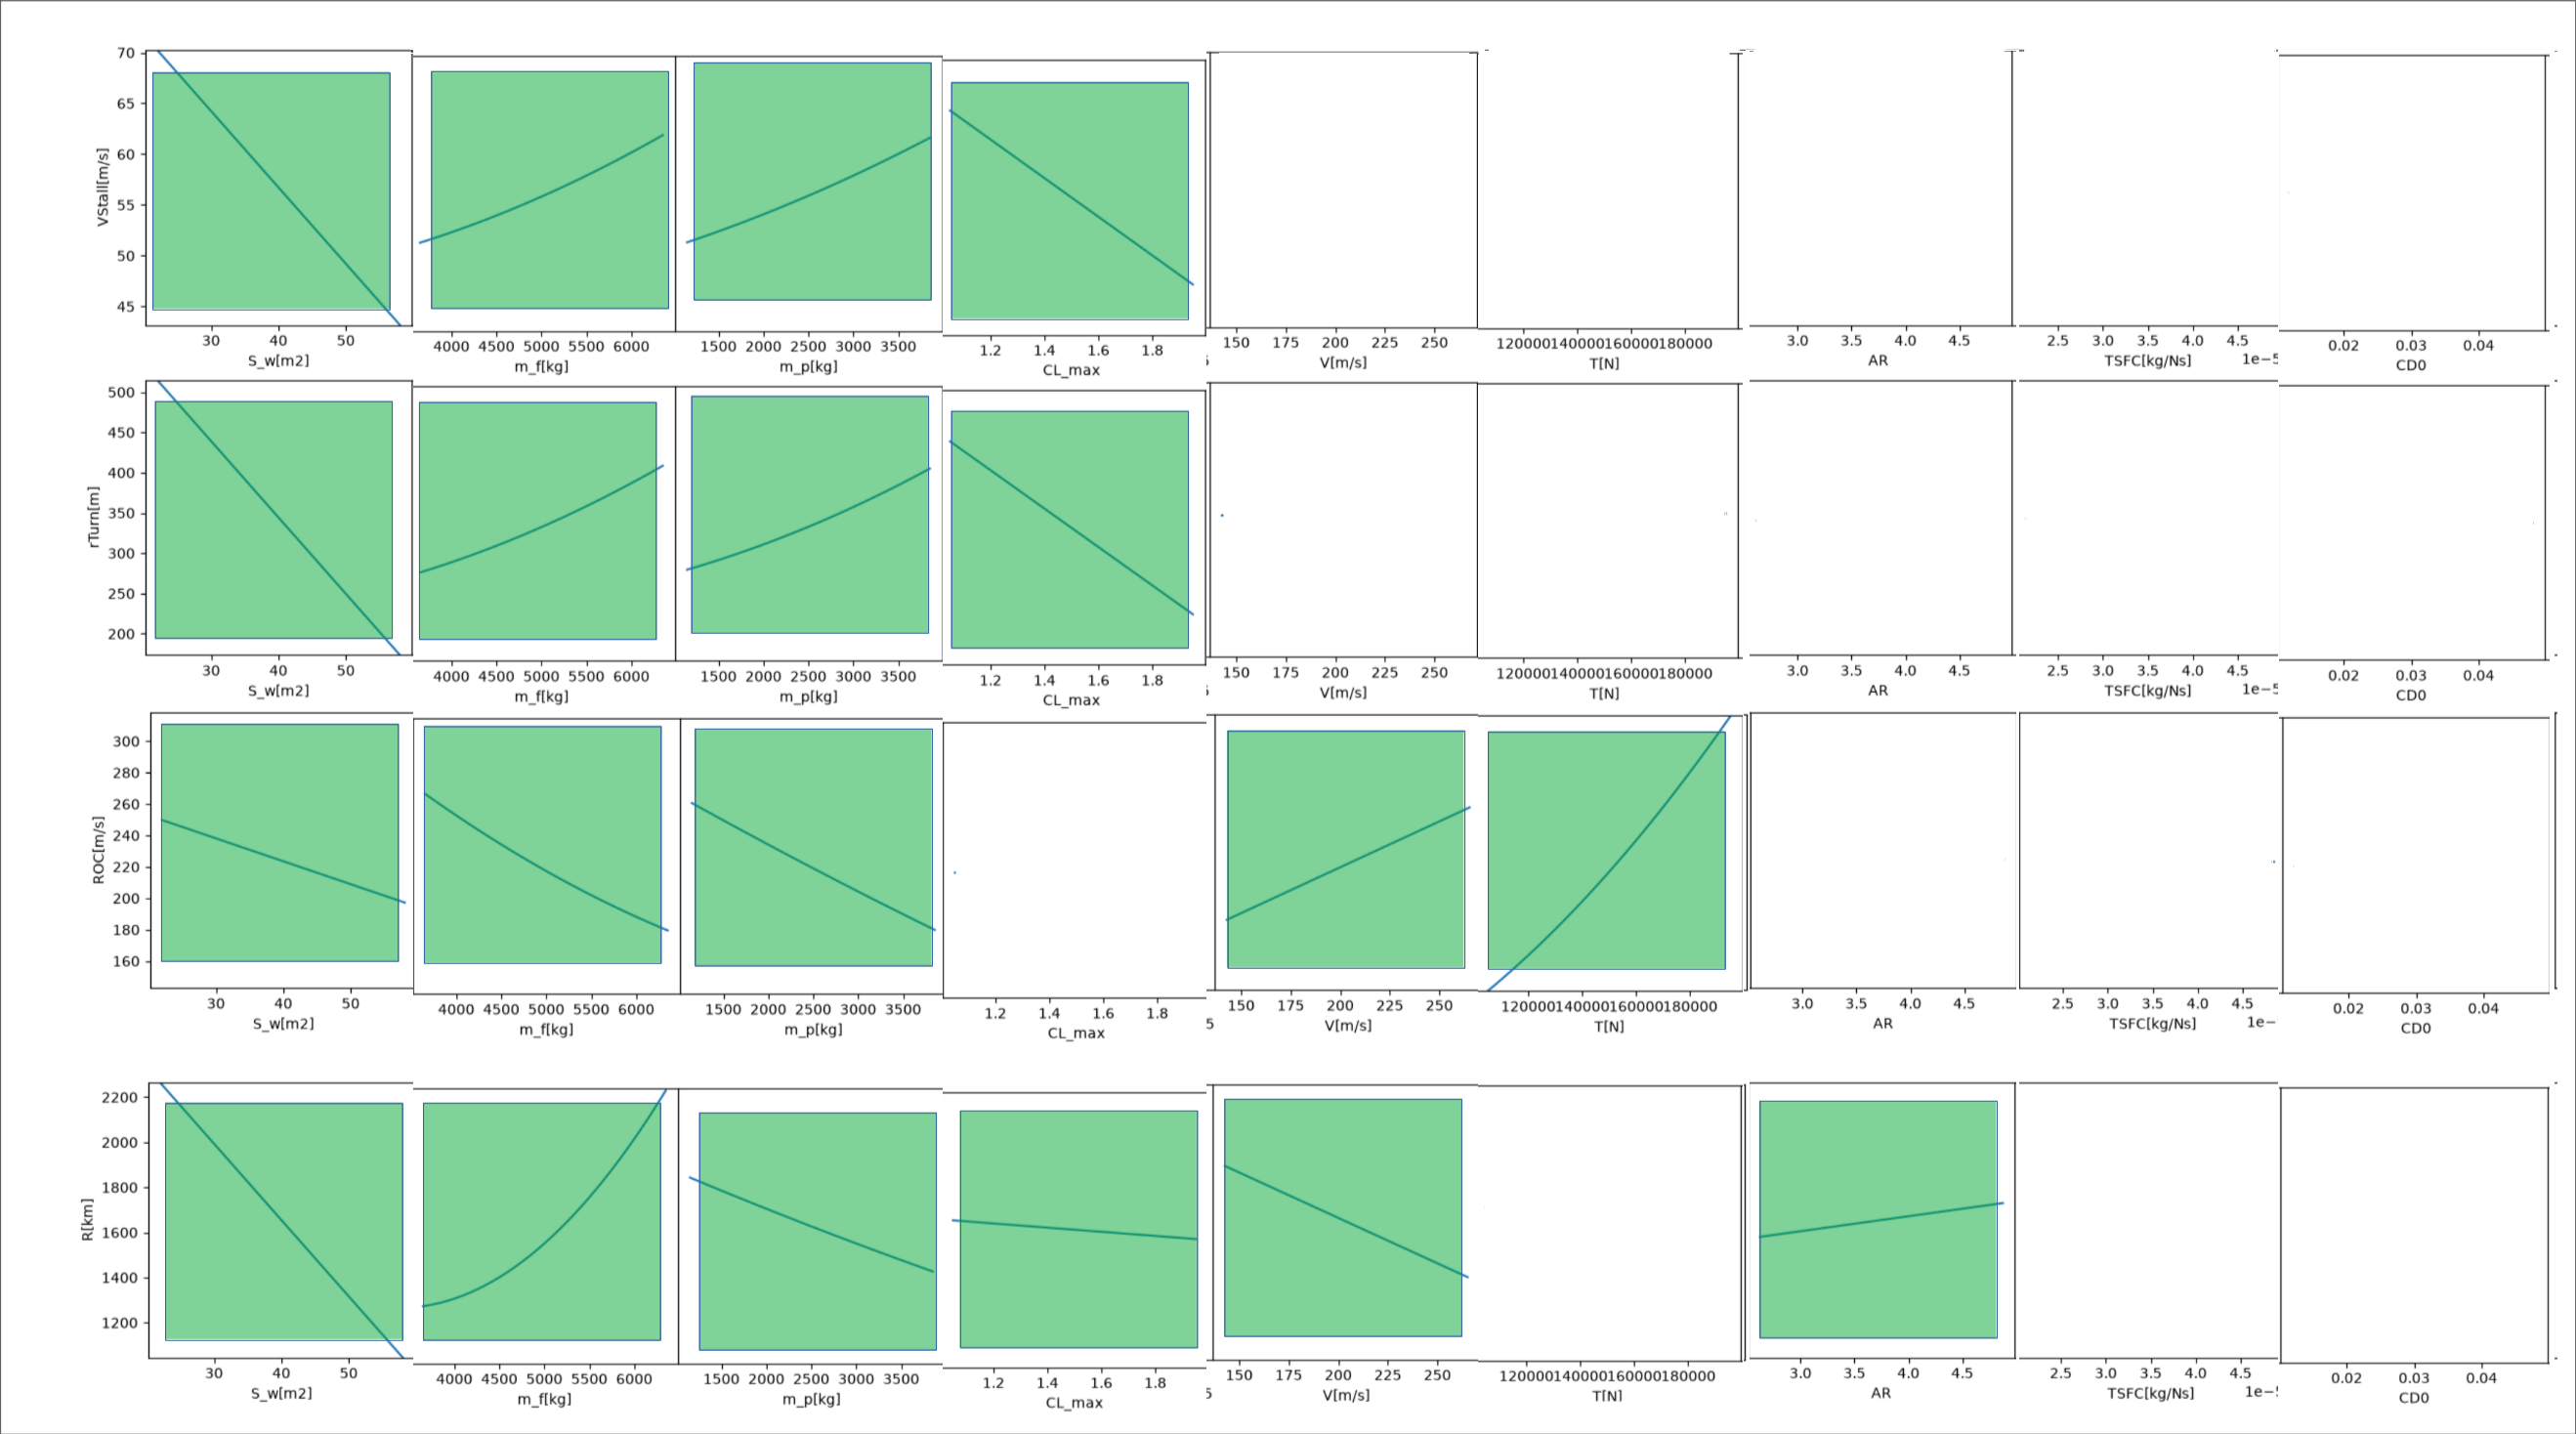
\includegraphics[width=\linewidth]{../UTIL/FIGS/axiomatic-matrix.png}
        \caption[width=.7\linewidth]{Sensitivity matrix post-ranking}
        \label{fig:AxiomaticMx}
\end{figure}

There are a few conclusions that can be drawn from this.
Firstly, TSFC and $C_{D0}$ have negligible impact on all of the DOs.
This implies that they are dominated by the other DVs in each DE.
It is possible that this is simply a feature of the response surface, with different bounds of the DVs having different sensitivities, but as the bounds are based on contemporary aircraft these DVs shall be discounted and fixed at their median value.
Secondly, $AR$ and $T$ only meaningfully affect one DO each.
This is important, as it means that they can be optimised by simply fixing the DV at the appropriate boundary: in this case, Thrust is set to $200 kN$ and AR set to 5.
Thirdly, increasing $m_{p}$ has a detrimental effect on all four DOs.
This is similar to $AR$ and $T$, in that it can be optimised by fixing it at the lowest bound ($1000 kg$).

This leaves four design variables with no clear option to fix.
In a decoupled system, there would always be a clear diagonal in a square matrix, making it easy to determine which DV should next be fixed.
Instead, as there is no diagonal and too many DVs to make a square matrix, a different approach must be taken.
In figure~\ref{fig:SM1}, there a few passing combinations of DVs (in blue).
This means that the orthotope of feasible designs exists within the current bounds.
To constrain the design space, the bounds for $S$ were set to the most extreme values that still passed, which were $31 \leq S \leq 58 \left[m^{2}\right]$.
From this point, each design variable's bounds were to be constrained to the extremes of the passing combinations iteratively until an entirely passing orthotope was seen.

\subsection{Design Trade-offs Visualisation}
As mentioned, the bounds of $S$ were reduced to $31 \leq S \leq 58 \left[m^{2}\right]$.
That resulted in figure~\ref{fig:R1}

\begin{figure}[H]
    \centering
        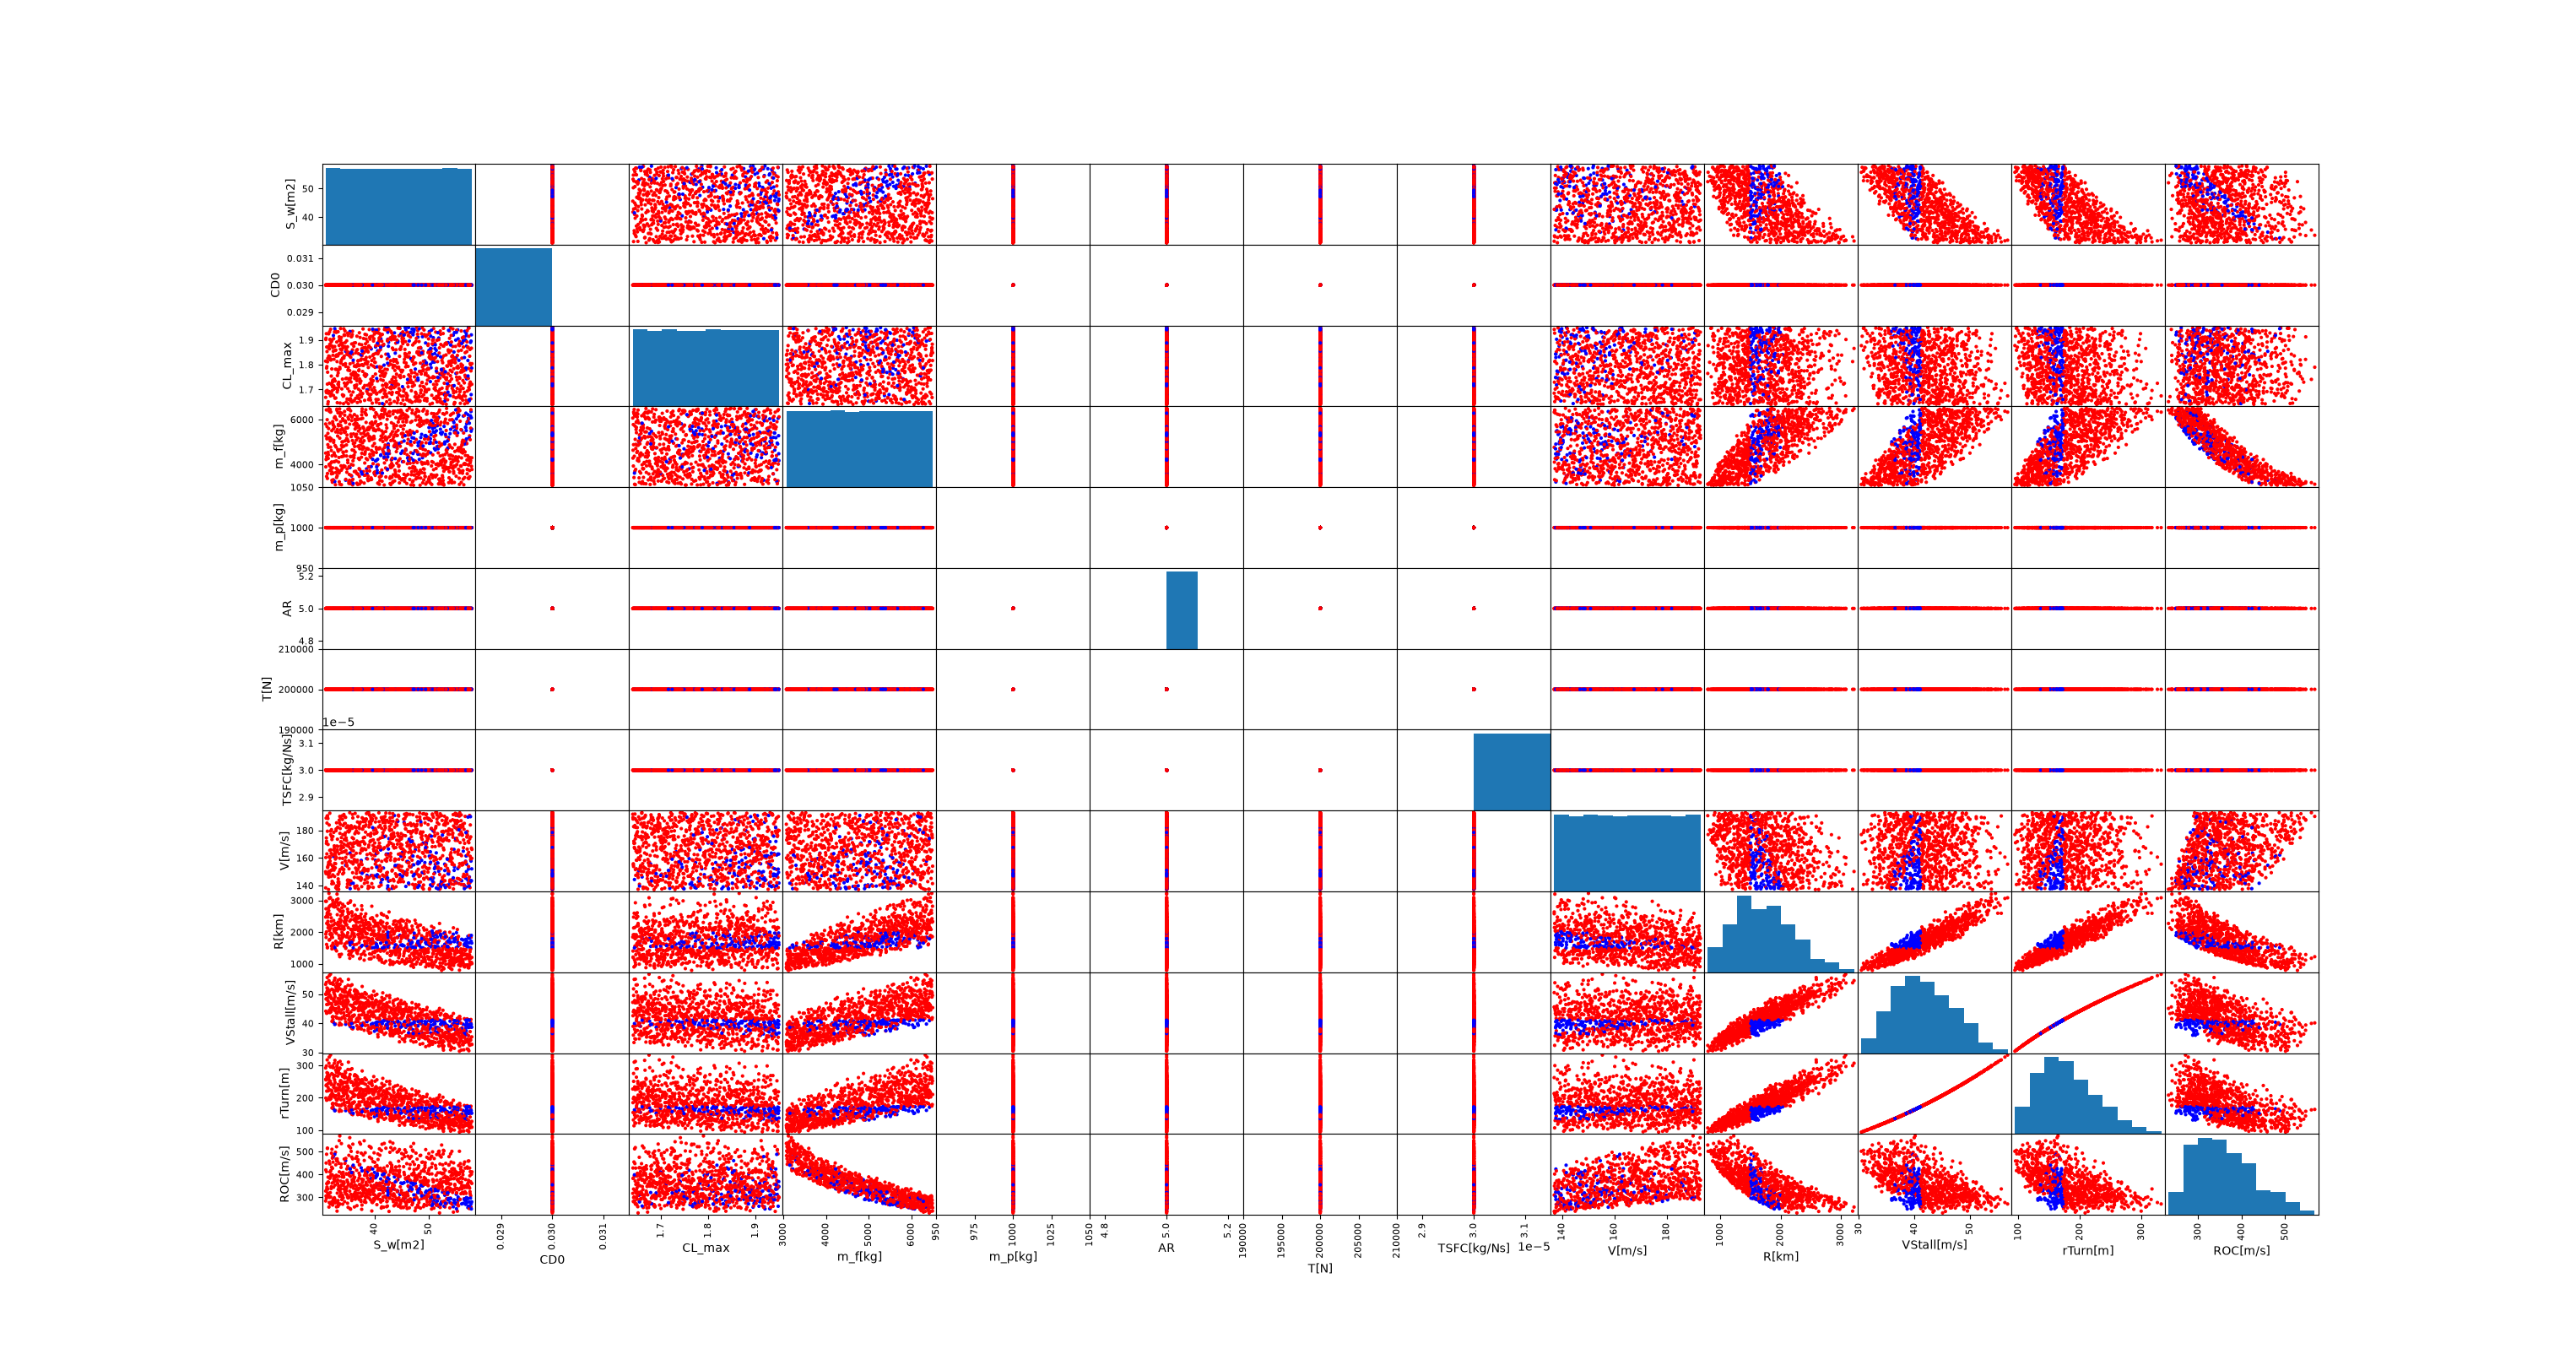
\includegraphics[width=1\linewidth]{../UTIL/FIGS/multiple-scatter-matrix-fixed-R1.png}
        \caption[width=.7\linewidth]{First round design space visualisaton with reduced $S$}
        \label{fig:R1}
\end{figure}

In the $S$ against $m_{f}$ plot, a diagonal band of passing values can be seen extending from the bottom left corner to the top right.
In the other plots, clouds of passes exist in the same space as failures.
As such, no simple bounds can be seen of a feasible orthotope.
The bounds of $m_f$ \textbf{and} $S$ were then reduced simultaneously, to focus in on a rectangle within the diagonal band, resulting in figure~\ref{fig:R2}


\begin{figure}[H]
    \centering
        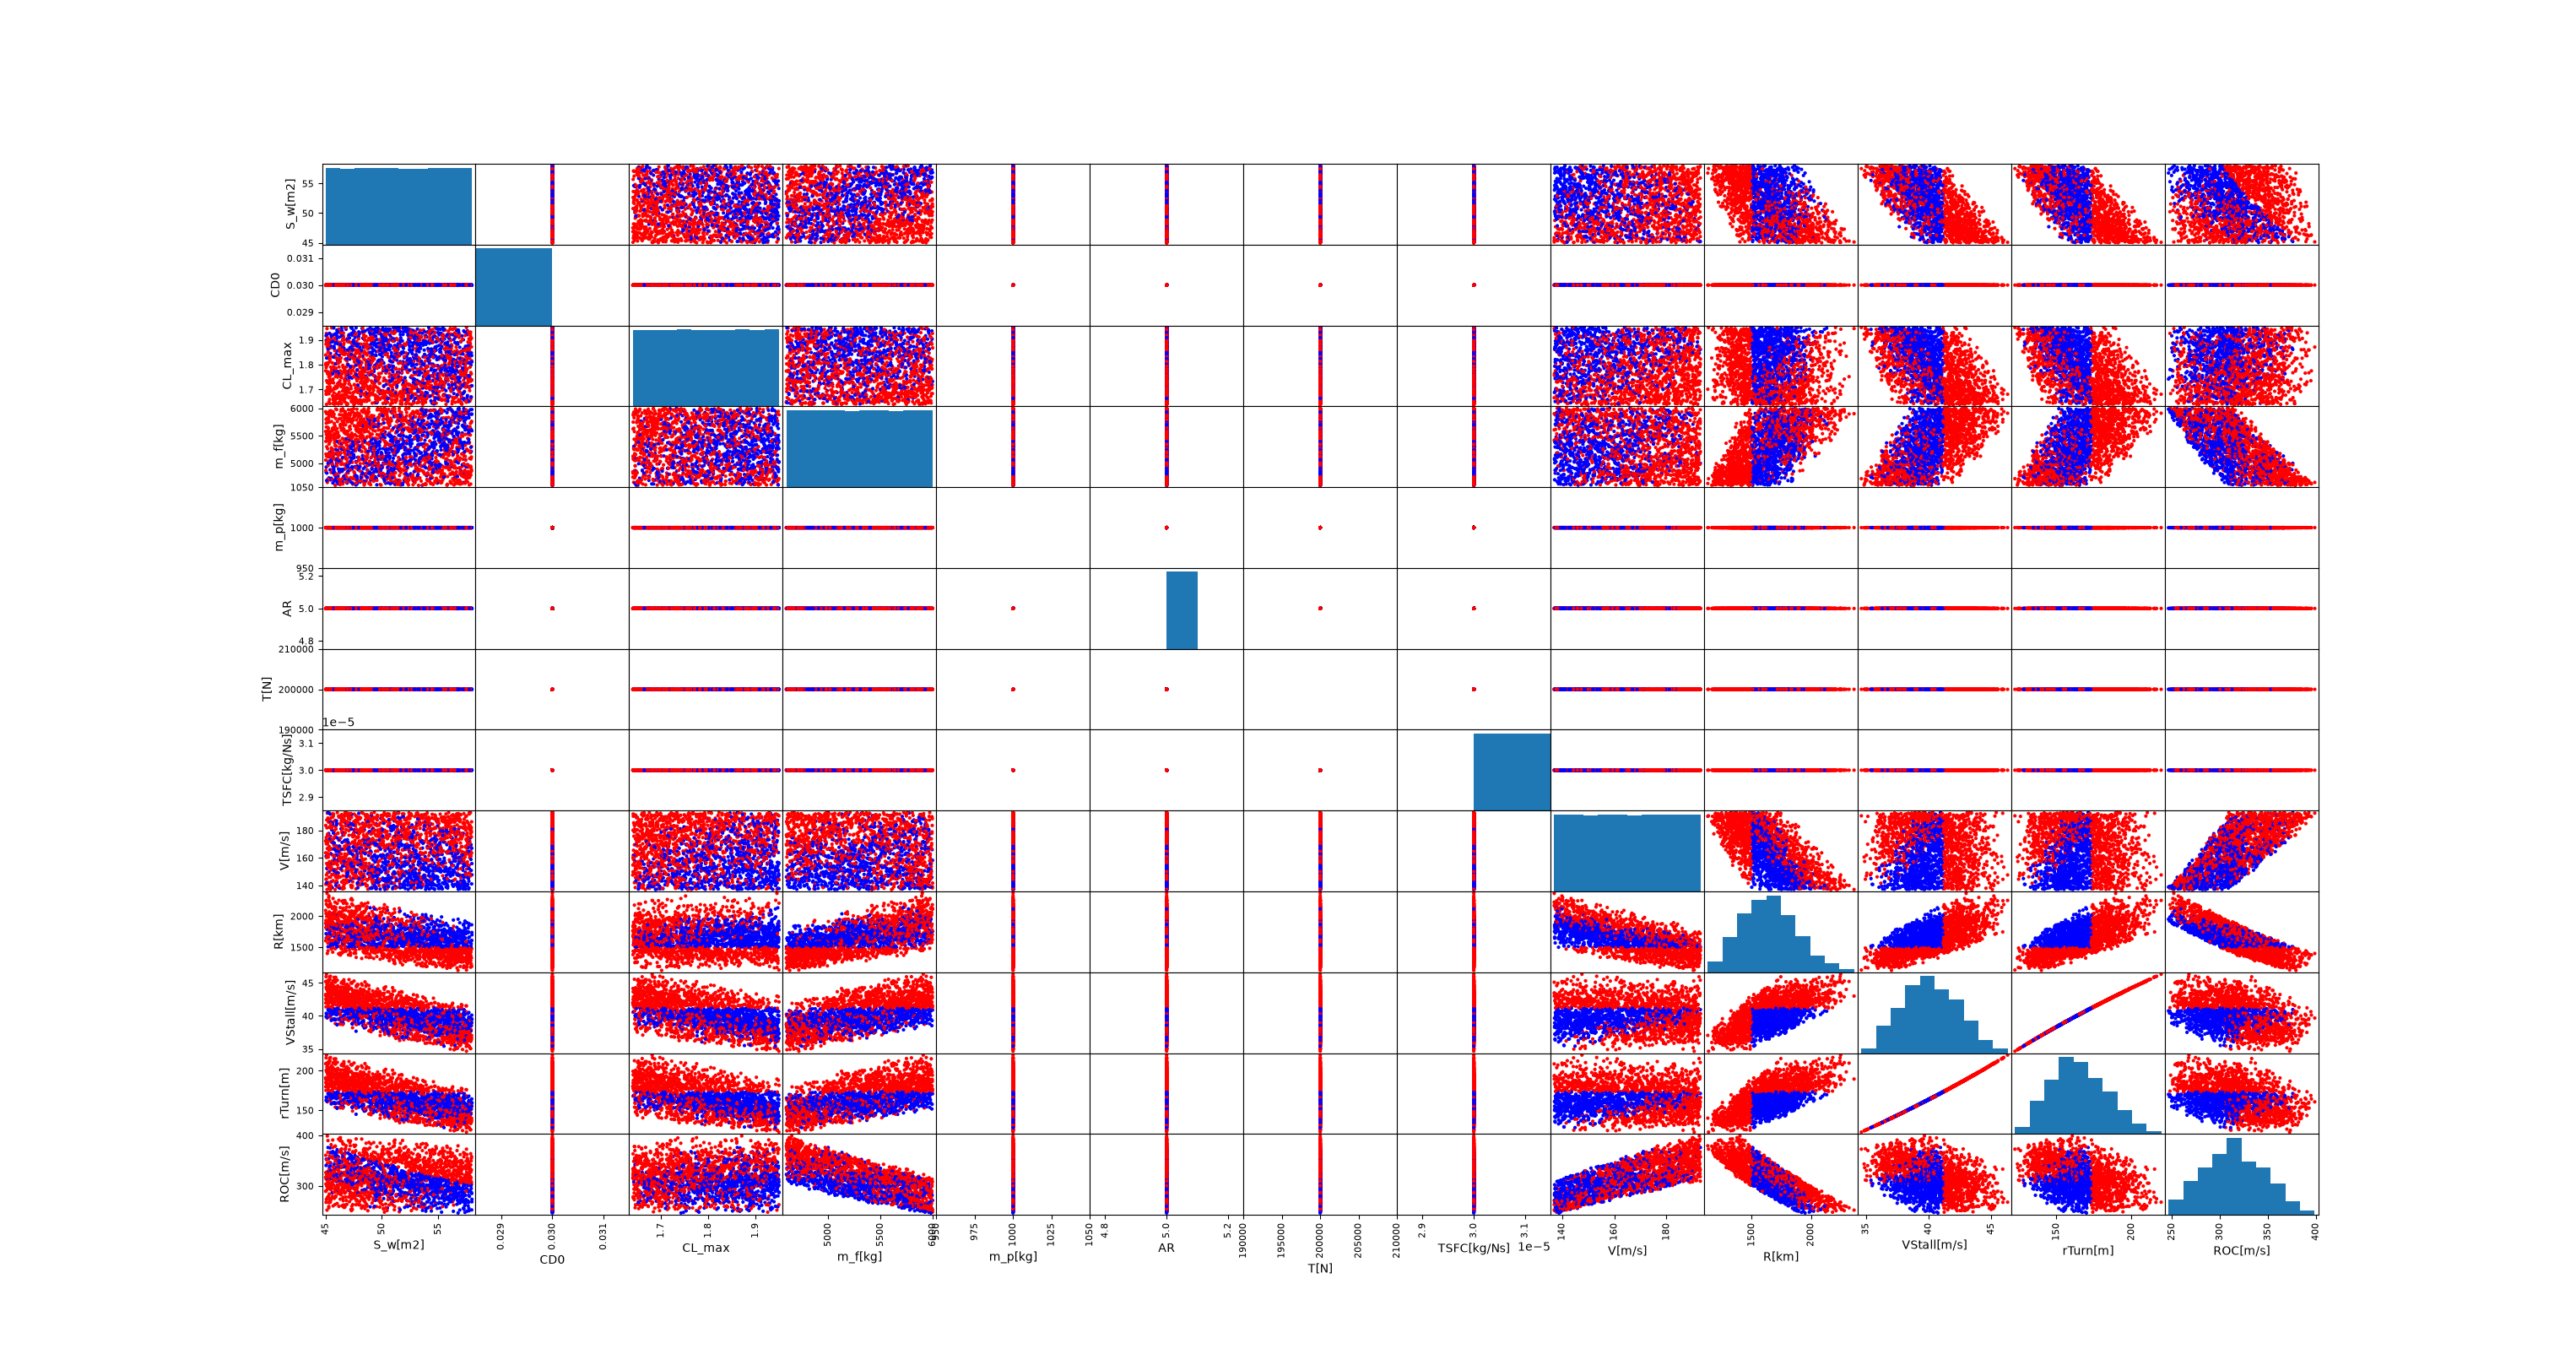
\includegraphics[width=\linewidth]{../UTIL/FIGS/multiple-scatter-matrix-fixed-R2-S-mf.png}
        \caption[width=.7\linewidth]{Second round design space visualisation with reduced $S$, $m_{f}$}
        \label{fig:R2}
\end{figure}

This process was repeated 6 times, with figures~\ref{fig:R3}-\ref{fig:R6} showing the stages of visualisation.

\begin{figure}[H]
    \centering
        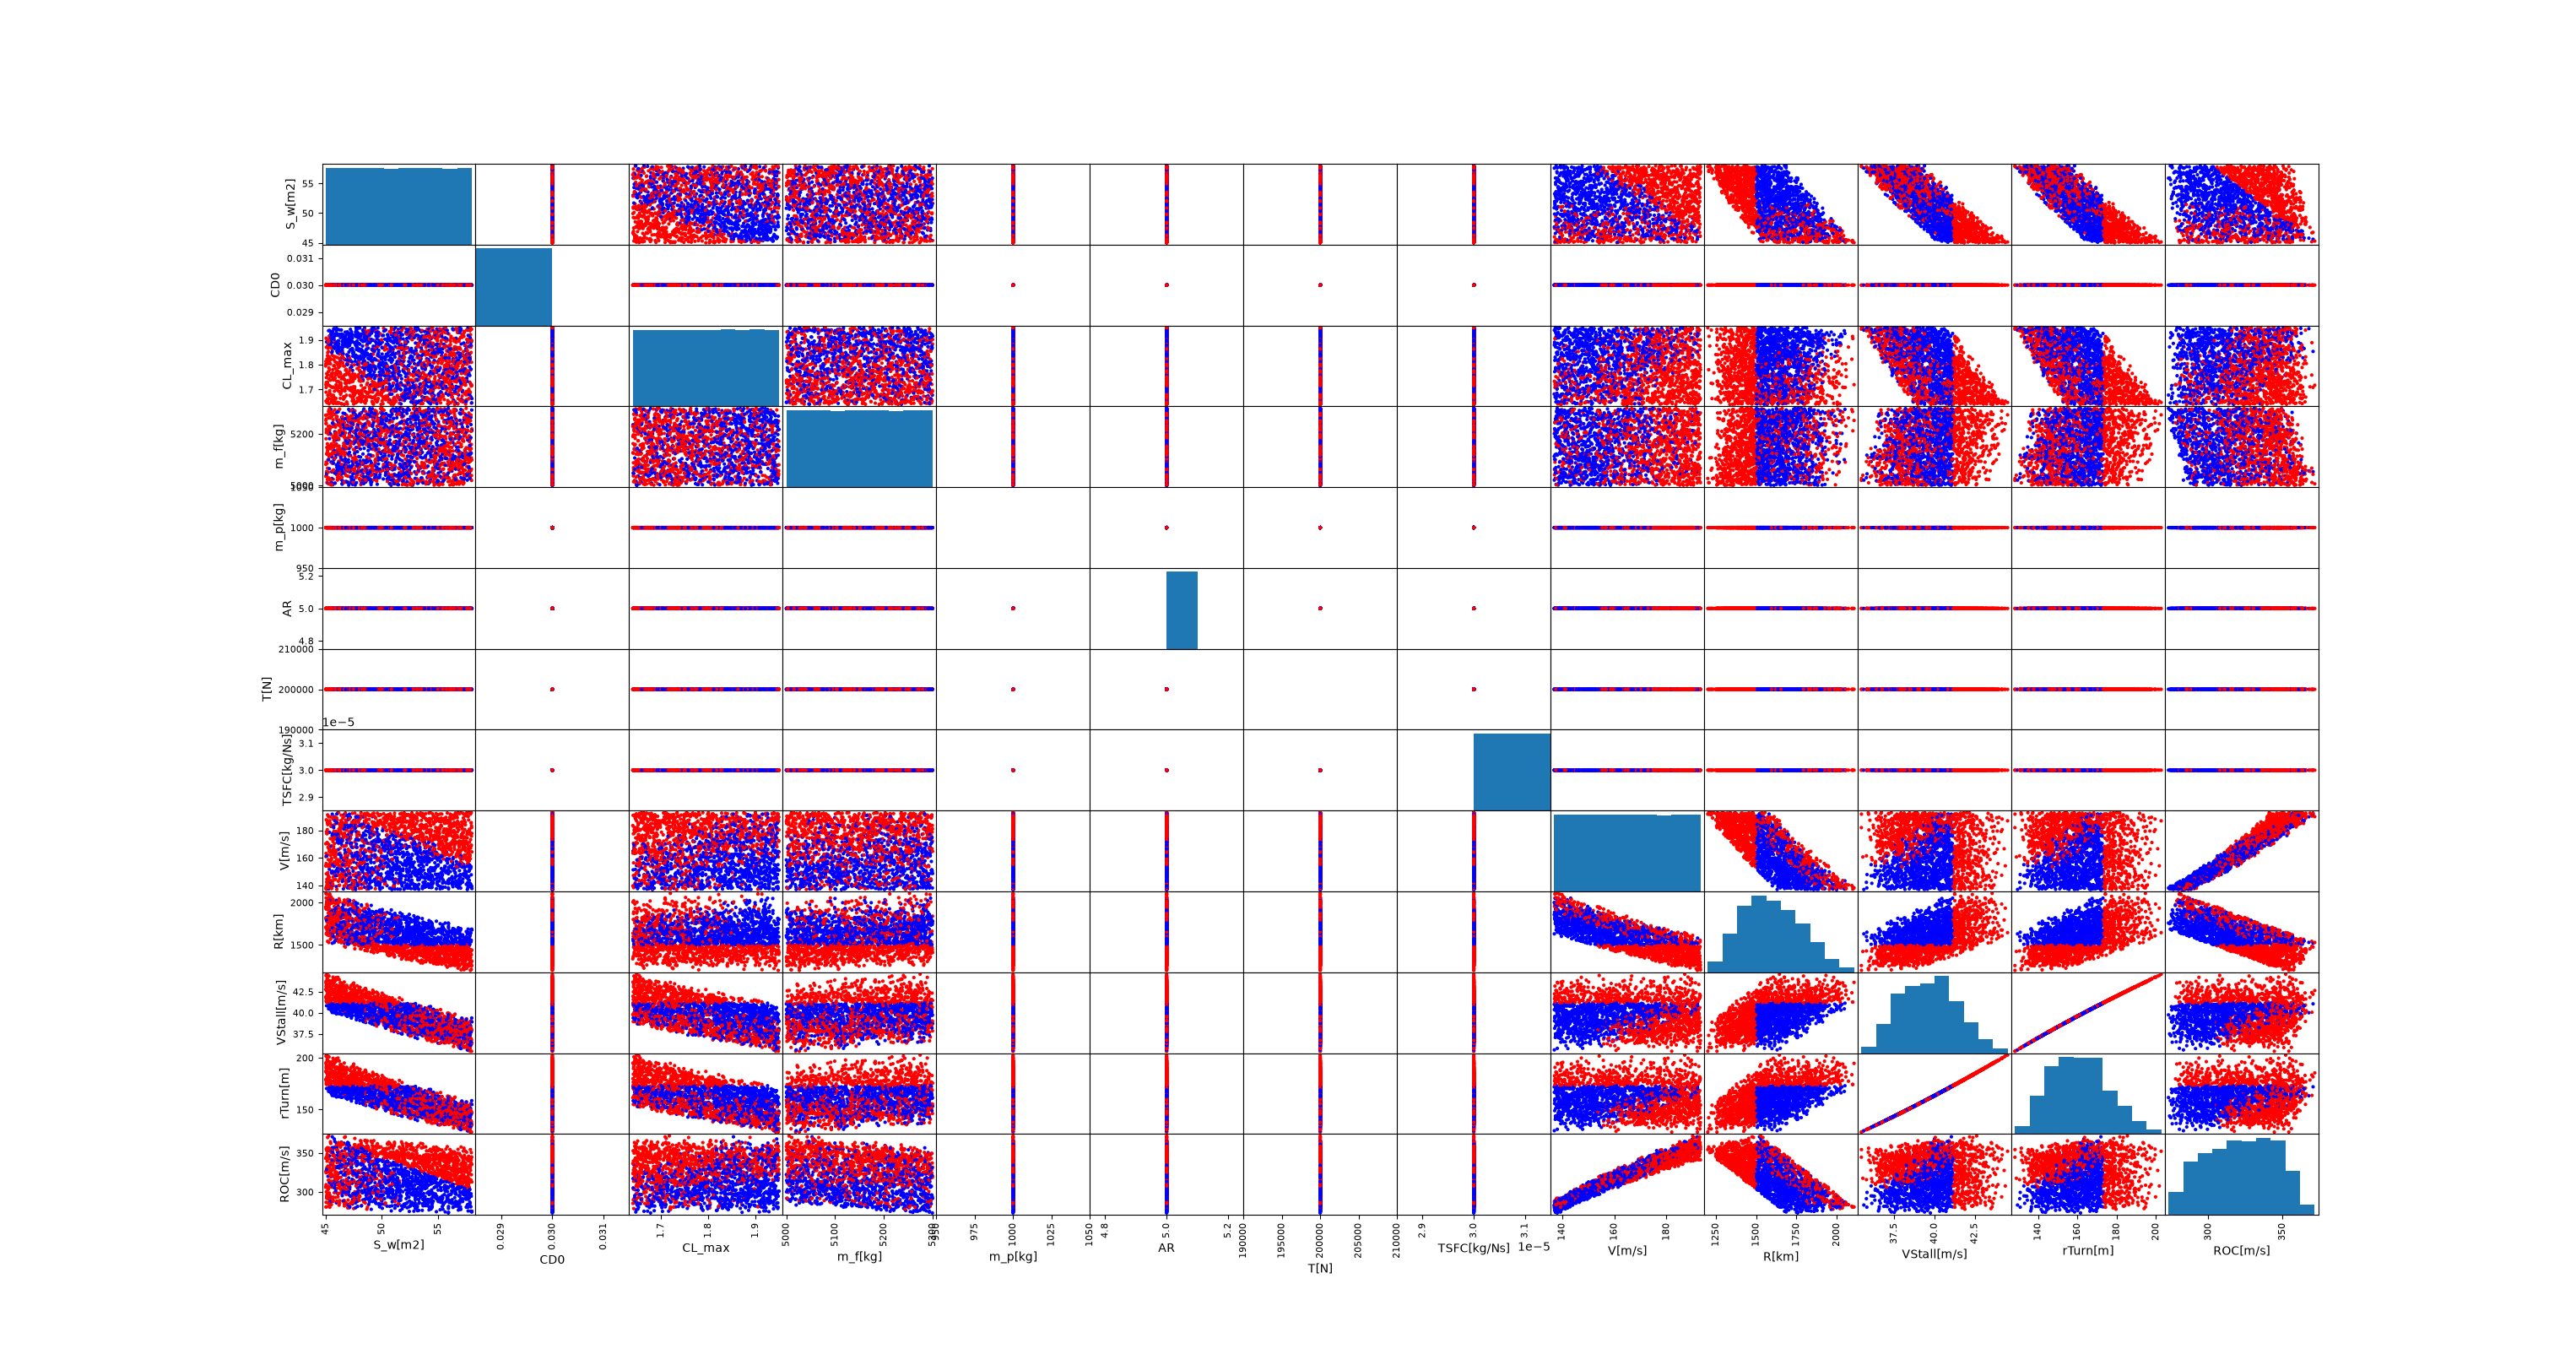
\includegraphics[width=\linewidth]{../UTIL/FIGS/multiple-scatter-matrix-fixed-R3-S-mf.png}
        \caption[width=.7\linewidth]{Third round design space visualisation with reduced $S$, $m_{f}$}
        \label{fig:R3}
\end{figure}

\begin{figure}[H]
    \centering
        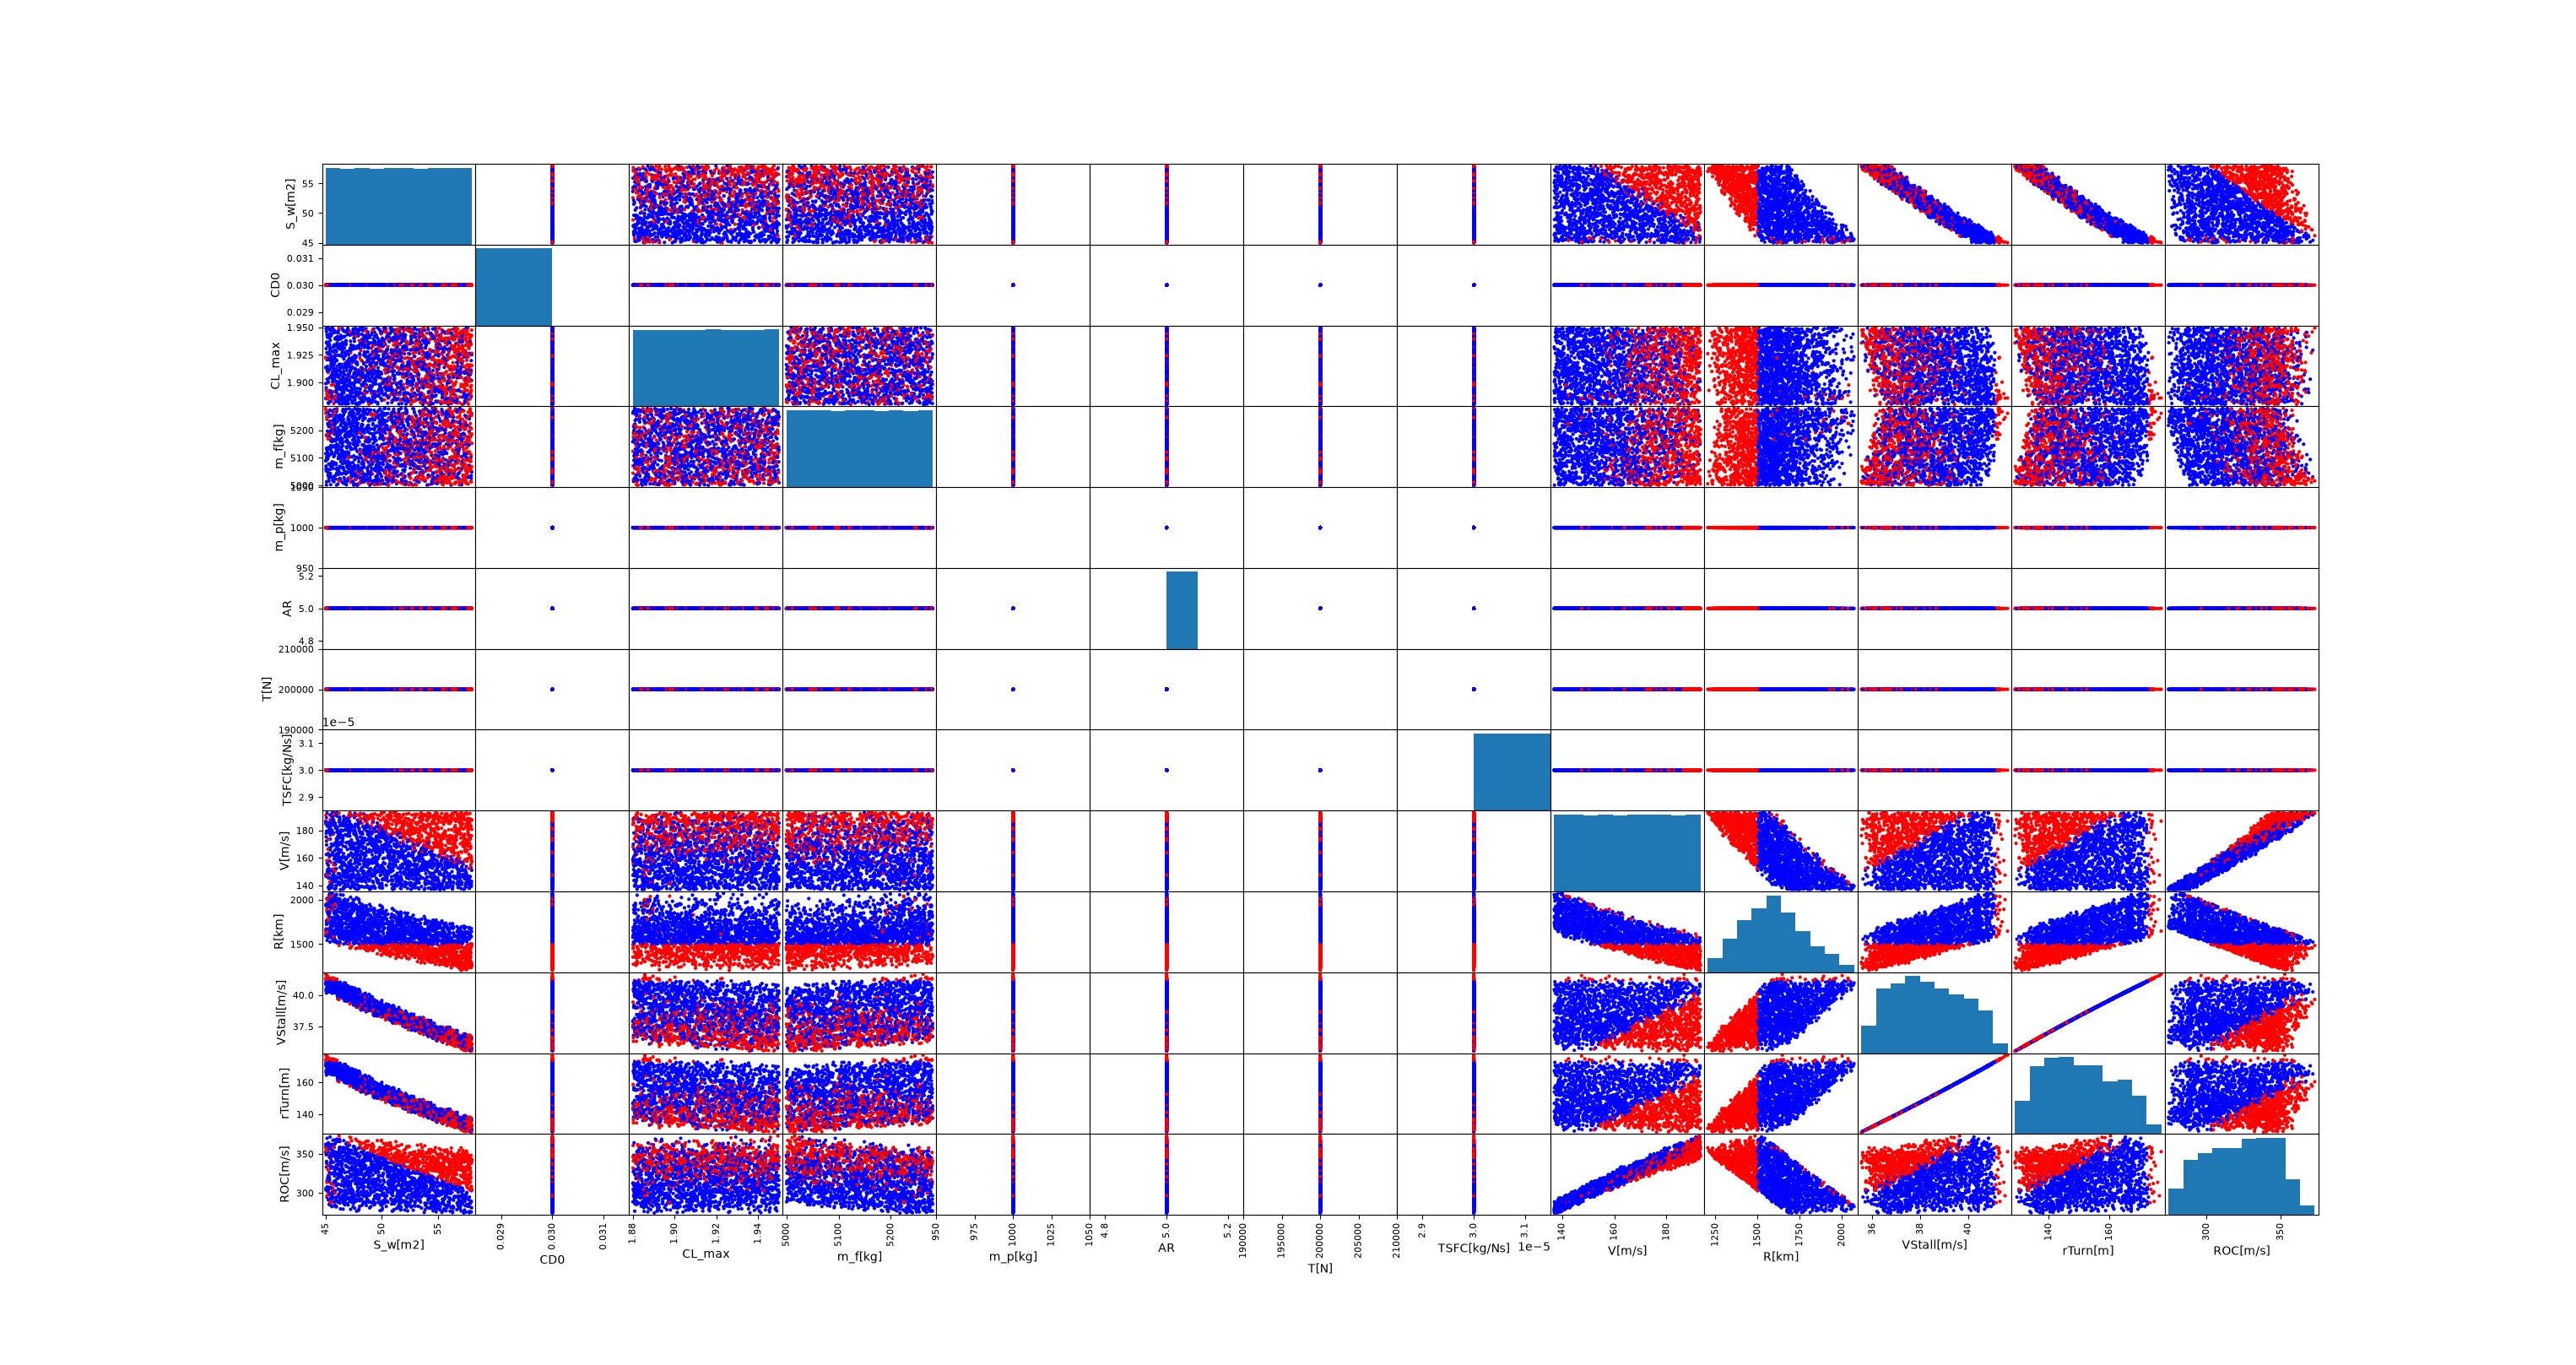
\includegraphics[width=\linewidth]{../UTIL/FIGS/multiple-scatter-matrix-fixed-R4-CL.png}
        \caption[width=.7\linewidth]{Fourth round design space visualisation with reduced $C_{Lmax}$}
        \label{fig:R4}
\end{figure}

\begin{figure}[H]
    \centering
        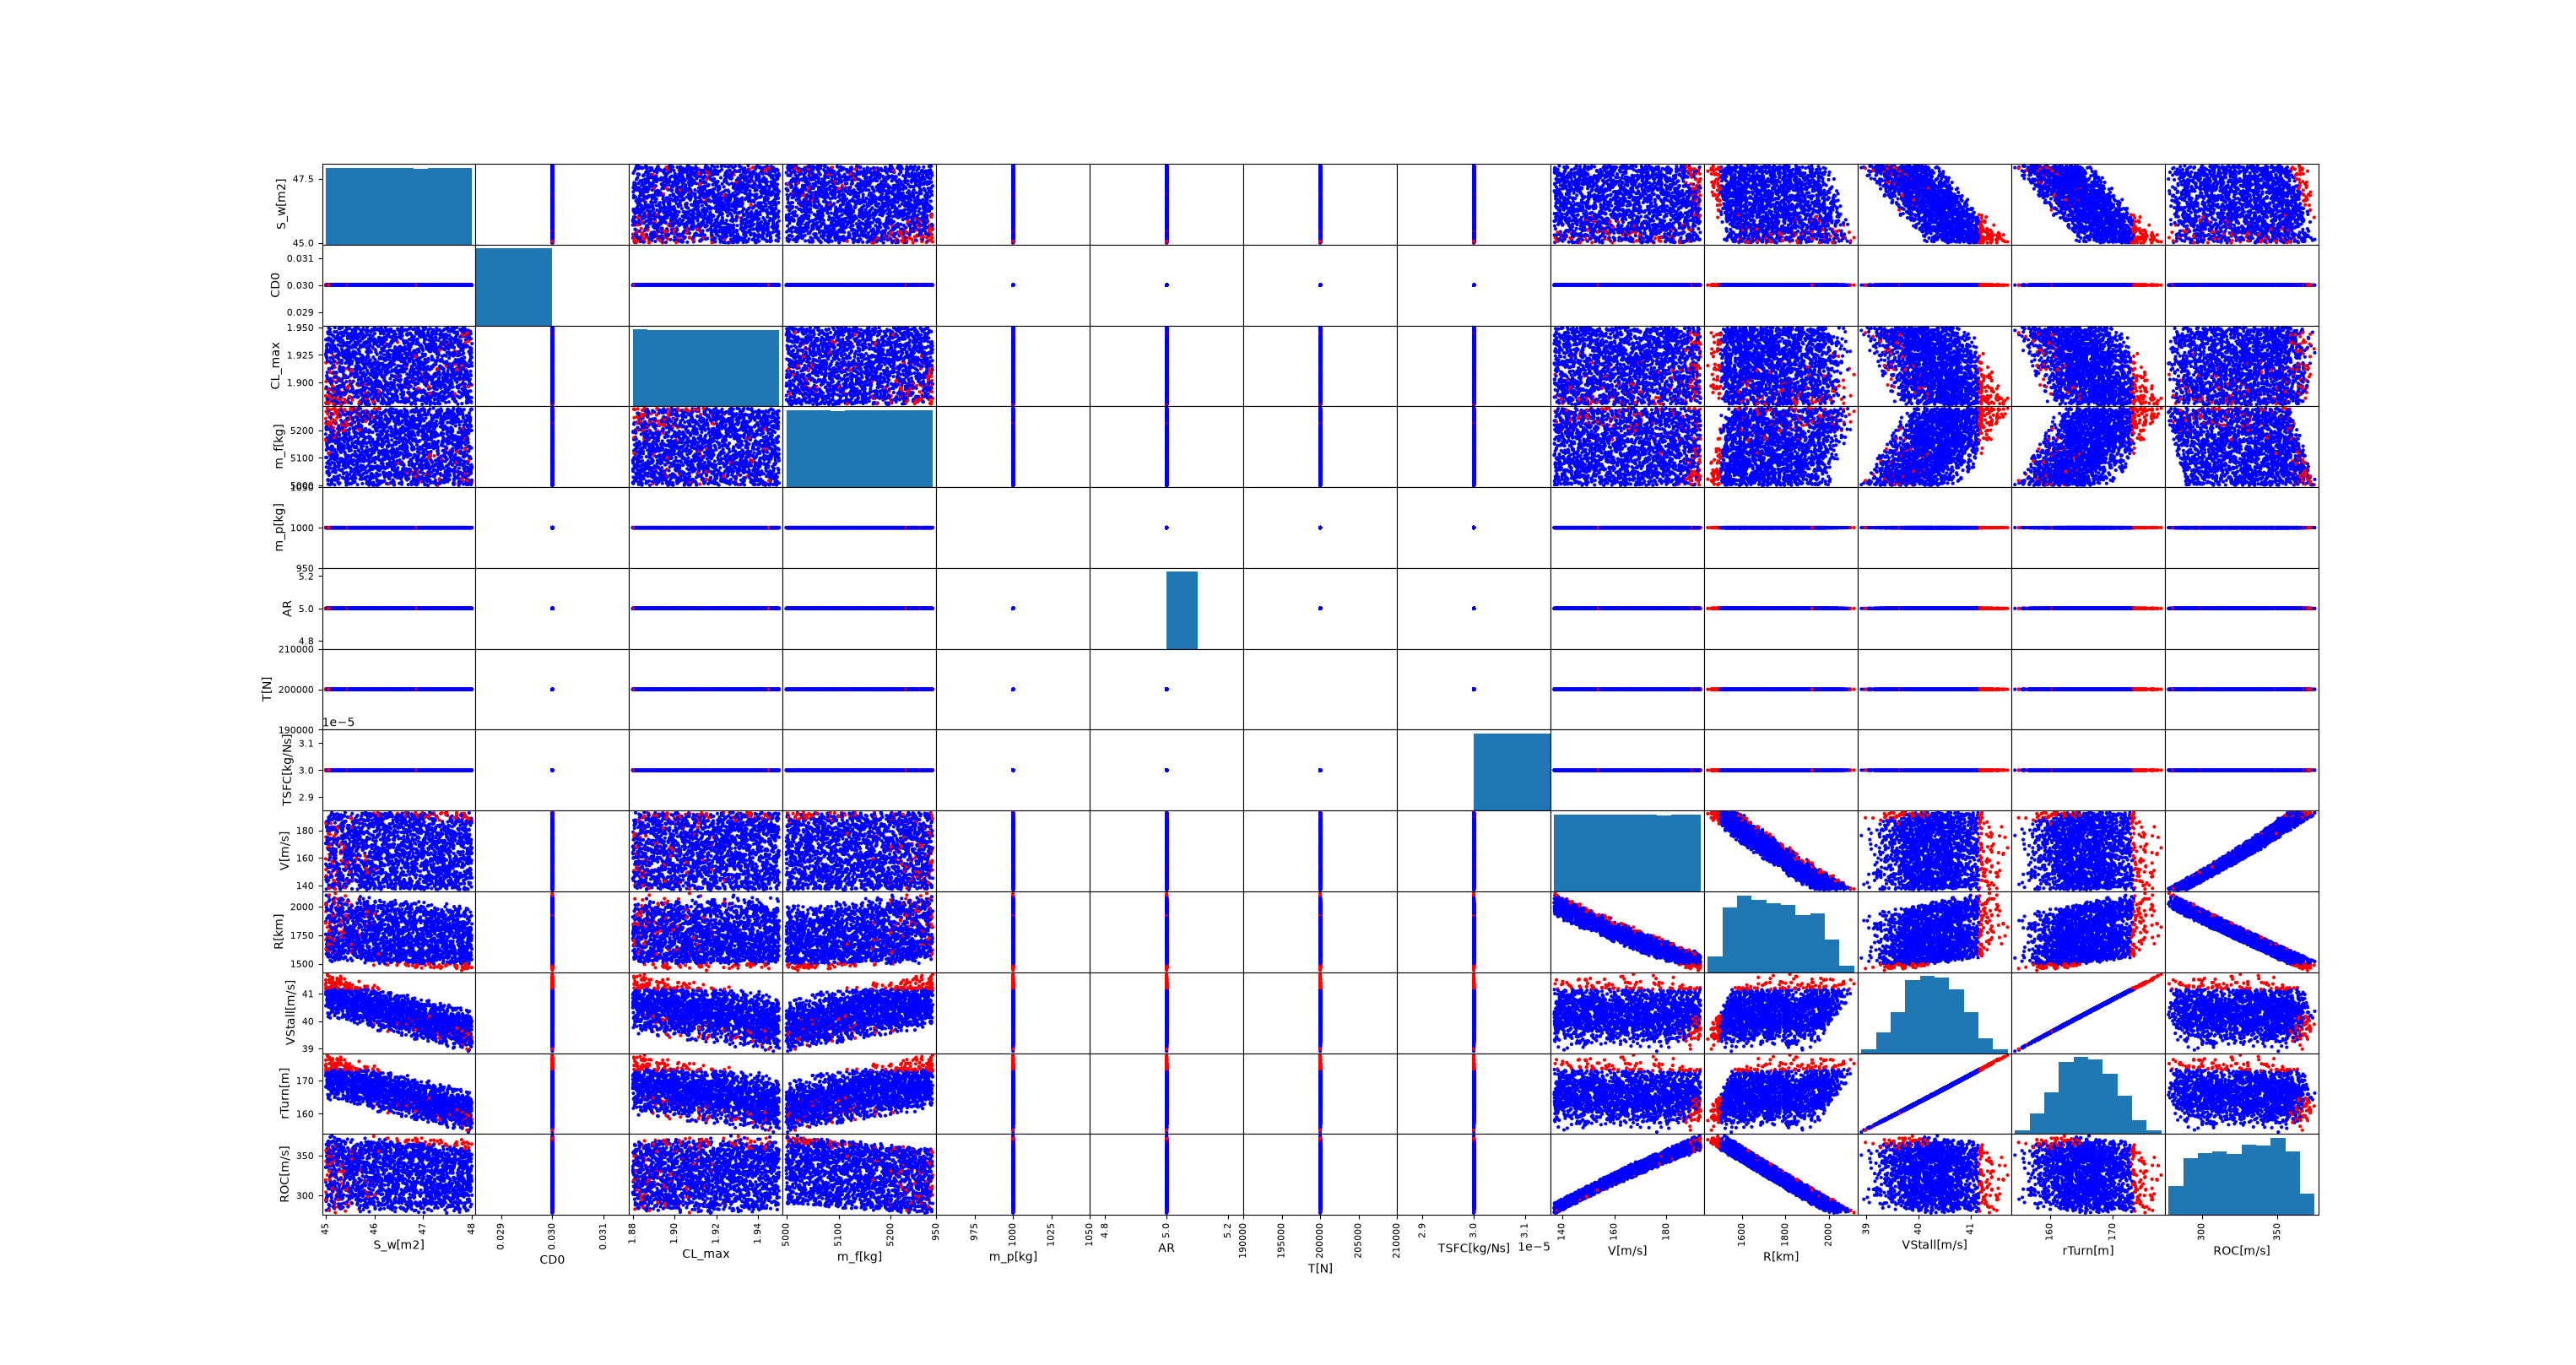
\includegraphics[width=\linewidth]{../UTIL/FIGS/multiple-scatter-matrix-fixed-R5-S.png}
        \caption[width=.7\linewidth]{Fifth round design space visualisation with reduced $S$}
        \label{fig:R5}
\end{figure}

\begin{figure}[H]
    \centering
        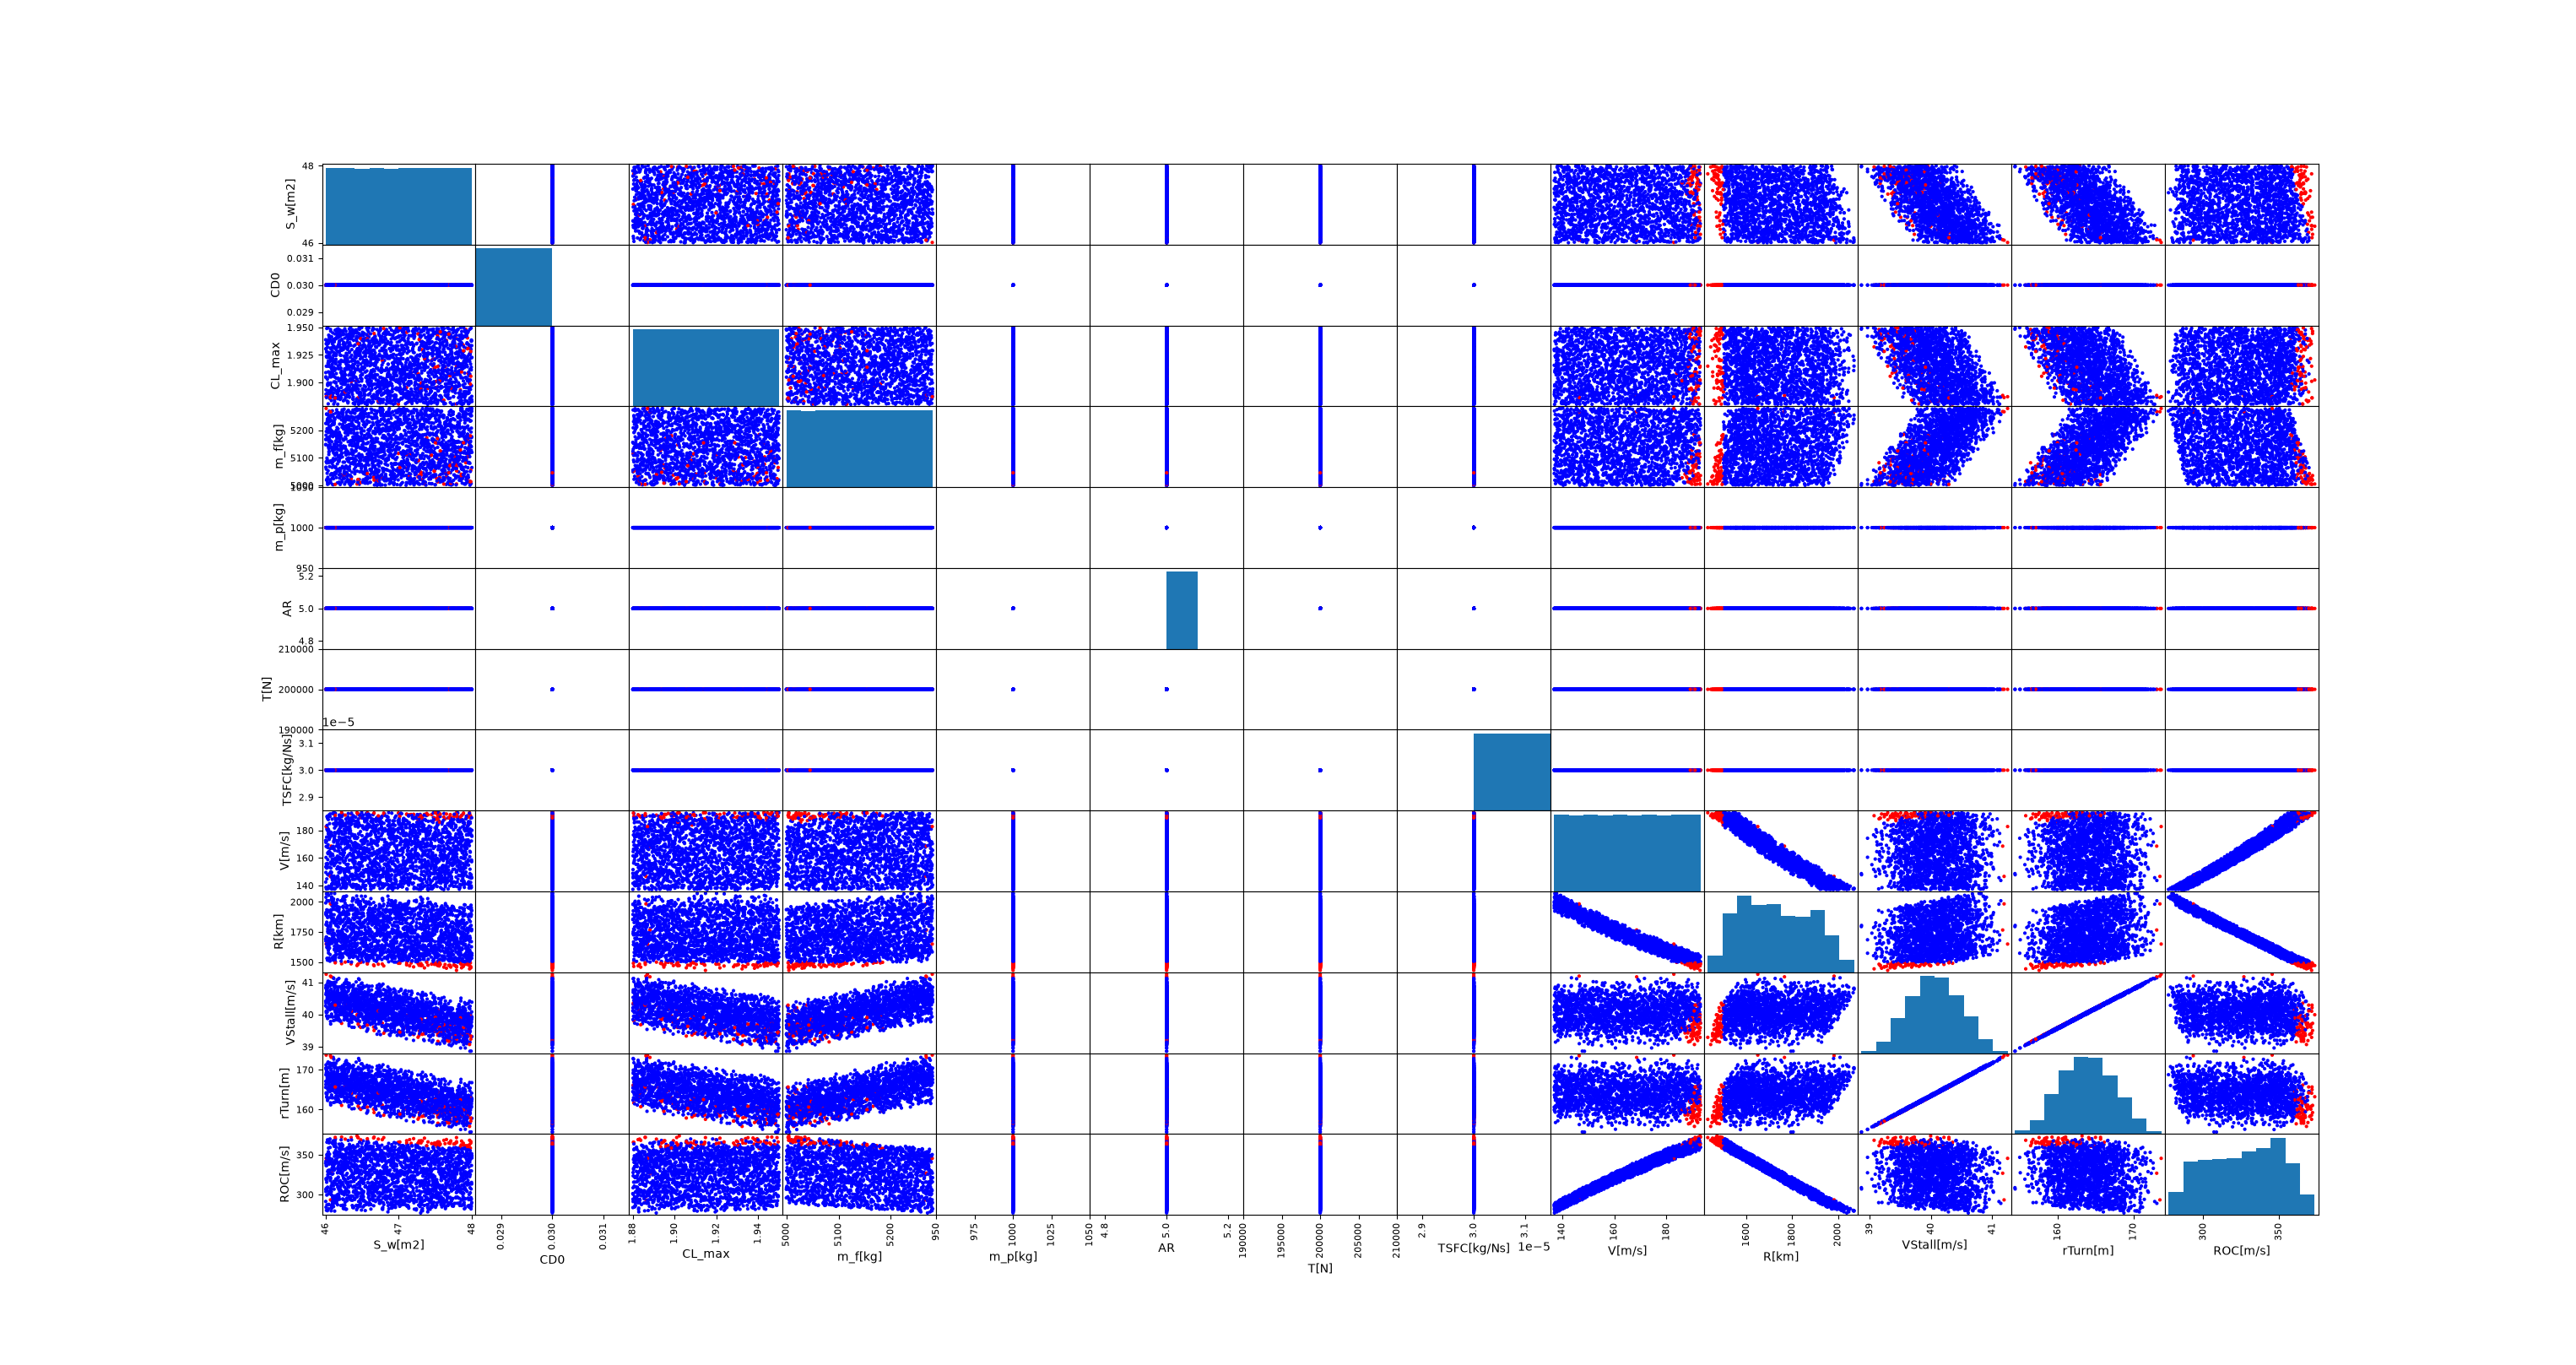
\includegraphics[width=\linewidth]{../UTIL/FIGS/multiple-scatter-matrix-fixed-R6-S.png}
        \caption[width=.7\linewidth]{Sixth round design space visualisation with reduced $S$}
        \label{fig:R6}
\end{figure}

At this point, a cluster of failures can be seen in the corners of the DV-DV plots.
They are intermixed with the passes, so there is no clear way to move the bounds to exclude them.
This implies that there is a part of the 4D orthotope that is extending into the failure region, and that it is being displayed unusually in 2D space.
Instead of attempting to cosntrain the orthotope, it was decided that $V$ be constrained to exclude the failing points, as it was the design variable with the greatest range between bounds remaining.
Additionally, the UCAV must perform across the flight envelope - constraining $V$ clearly implies that the design is non compliant.
Instead, future work would argue that the performance requirements are too stringent for the entire flight envelope, and negotiate a compromise where the requirements are relaxed either across the envelope, or only for the regions where the designs are infeasible.
This constraint results in figure~\ref{fig:Orthotope} with no failures.

\begin{figure}[H]
    \centering
        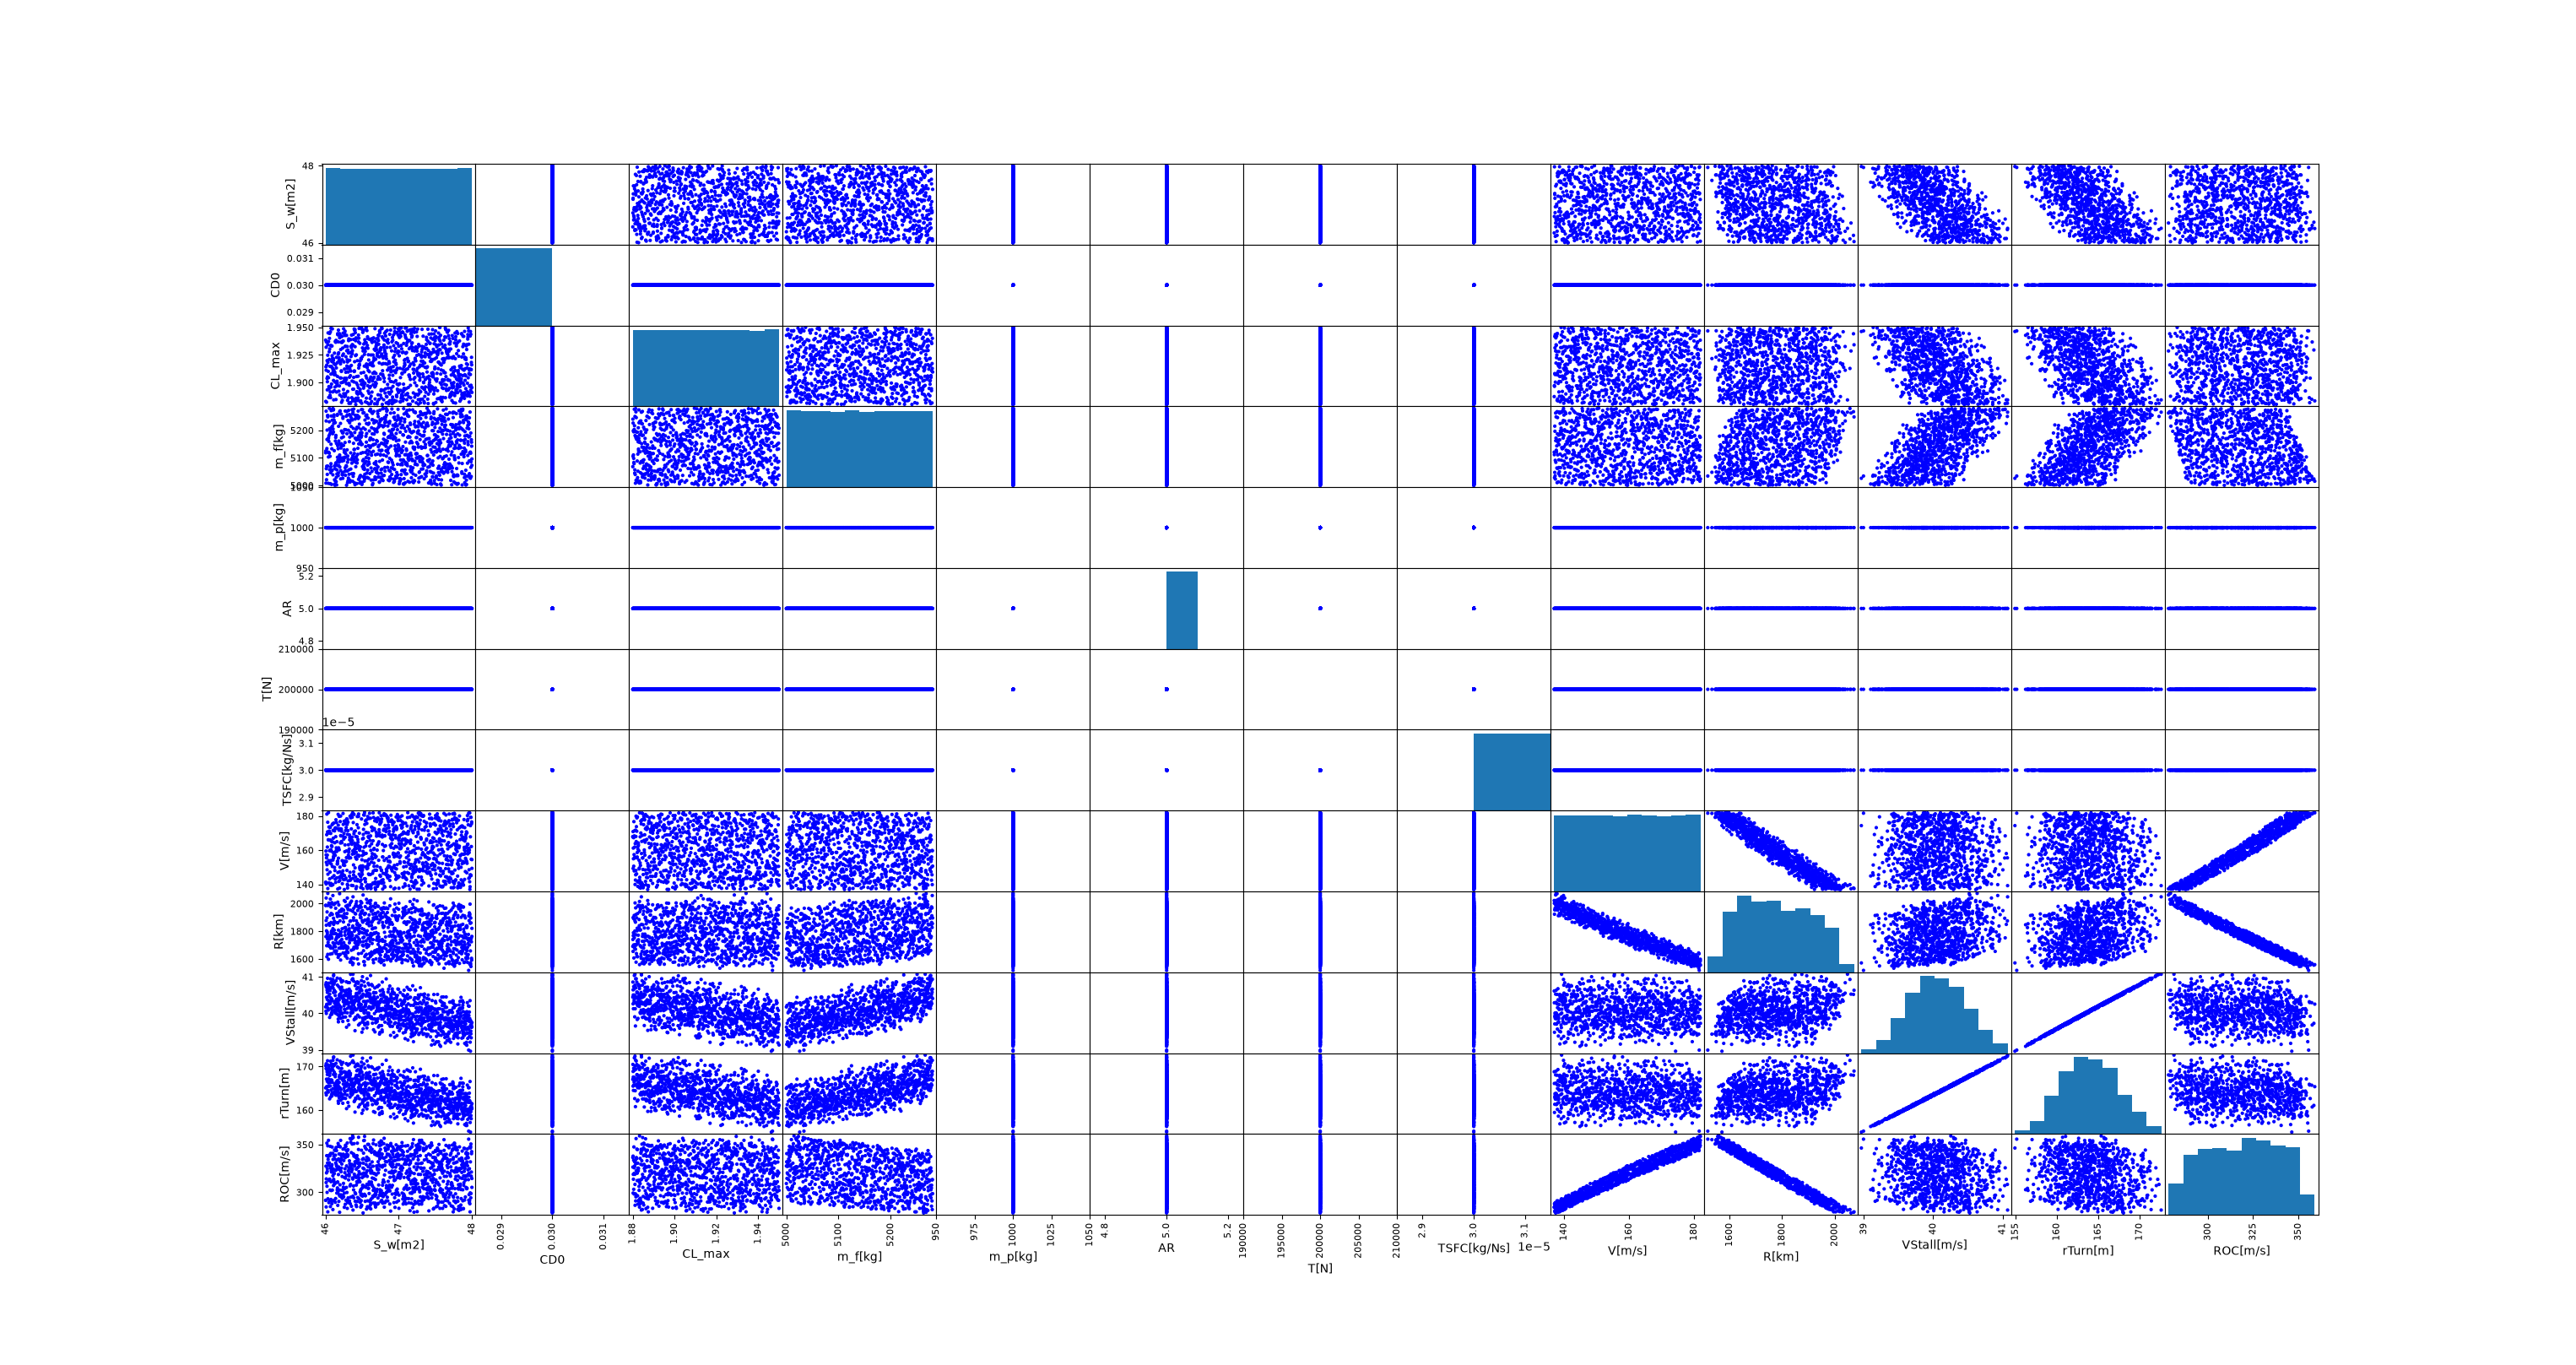
\includegraphics[width=\linewidth]{../UTIL/FIGS/multiple-scatter-matrix-orthotope.png}
        \caption[width=.7\linewidth]{Final design space visualisation with final bounds set}
        \label{fig:Orthotope}
\end{figure}

\subsection{Design Trade-offs Analysis}

Now that a feasibility region has been defined, it is possible to determine the final solution specification.
There are two methods of achieving this, that are determined by whether or not there is preference in DVs or in DOs.
In this early stage, there is no clear preference in DVs.
All of variables are free to move within their bounds, and there are no requirements forcing any to be minimised/maximised.
This is a feature of the restricted requirements set and the requirement rankings, as introducing cost, efficiency, or weapons loadout would almost certainly have implications for the DVs.
As it stands, though, no DV is preferred over another, but there is preference in the DOs.
It would be possible to determine which performance requirements are derived from the most capabilities, but as the CAP capability is so much more preferred, selecting the most important DO to enable that is more suitable.
On the assumption that the majority of the time a combat air patrol will not encounter hostile aircraft, the most important objective is range; range is considered on every sortie, not only those where combat occurs.

As such, a heuristic search for optimal values was performed.
This was done with a multi-objective optimisation genetic algorithm, implemented by the pymoo module.
Pymoo has many available algorithms, but for this optimisation NSGA-II was chosen.
This was implemented in the \texttt{/new-bounds/optimiseMultiple-orthotope.py} script, which performs 2000 iterations on a population size of 200.
This produced a Pareto-optimal front of DVs, which was then coloured by the resultant Range.
See figure~\ref{fig:paretoDV}.
This script also output the design with the greatest range.

\begin{figure}[H]
    \centering
        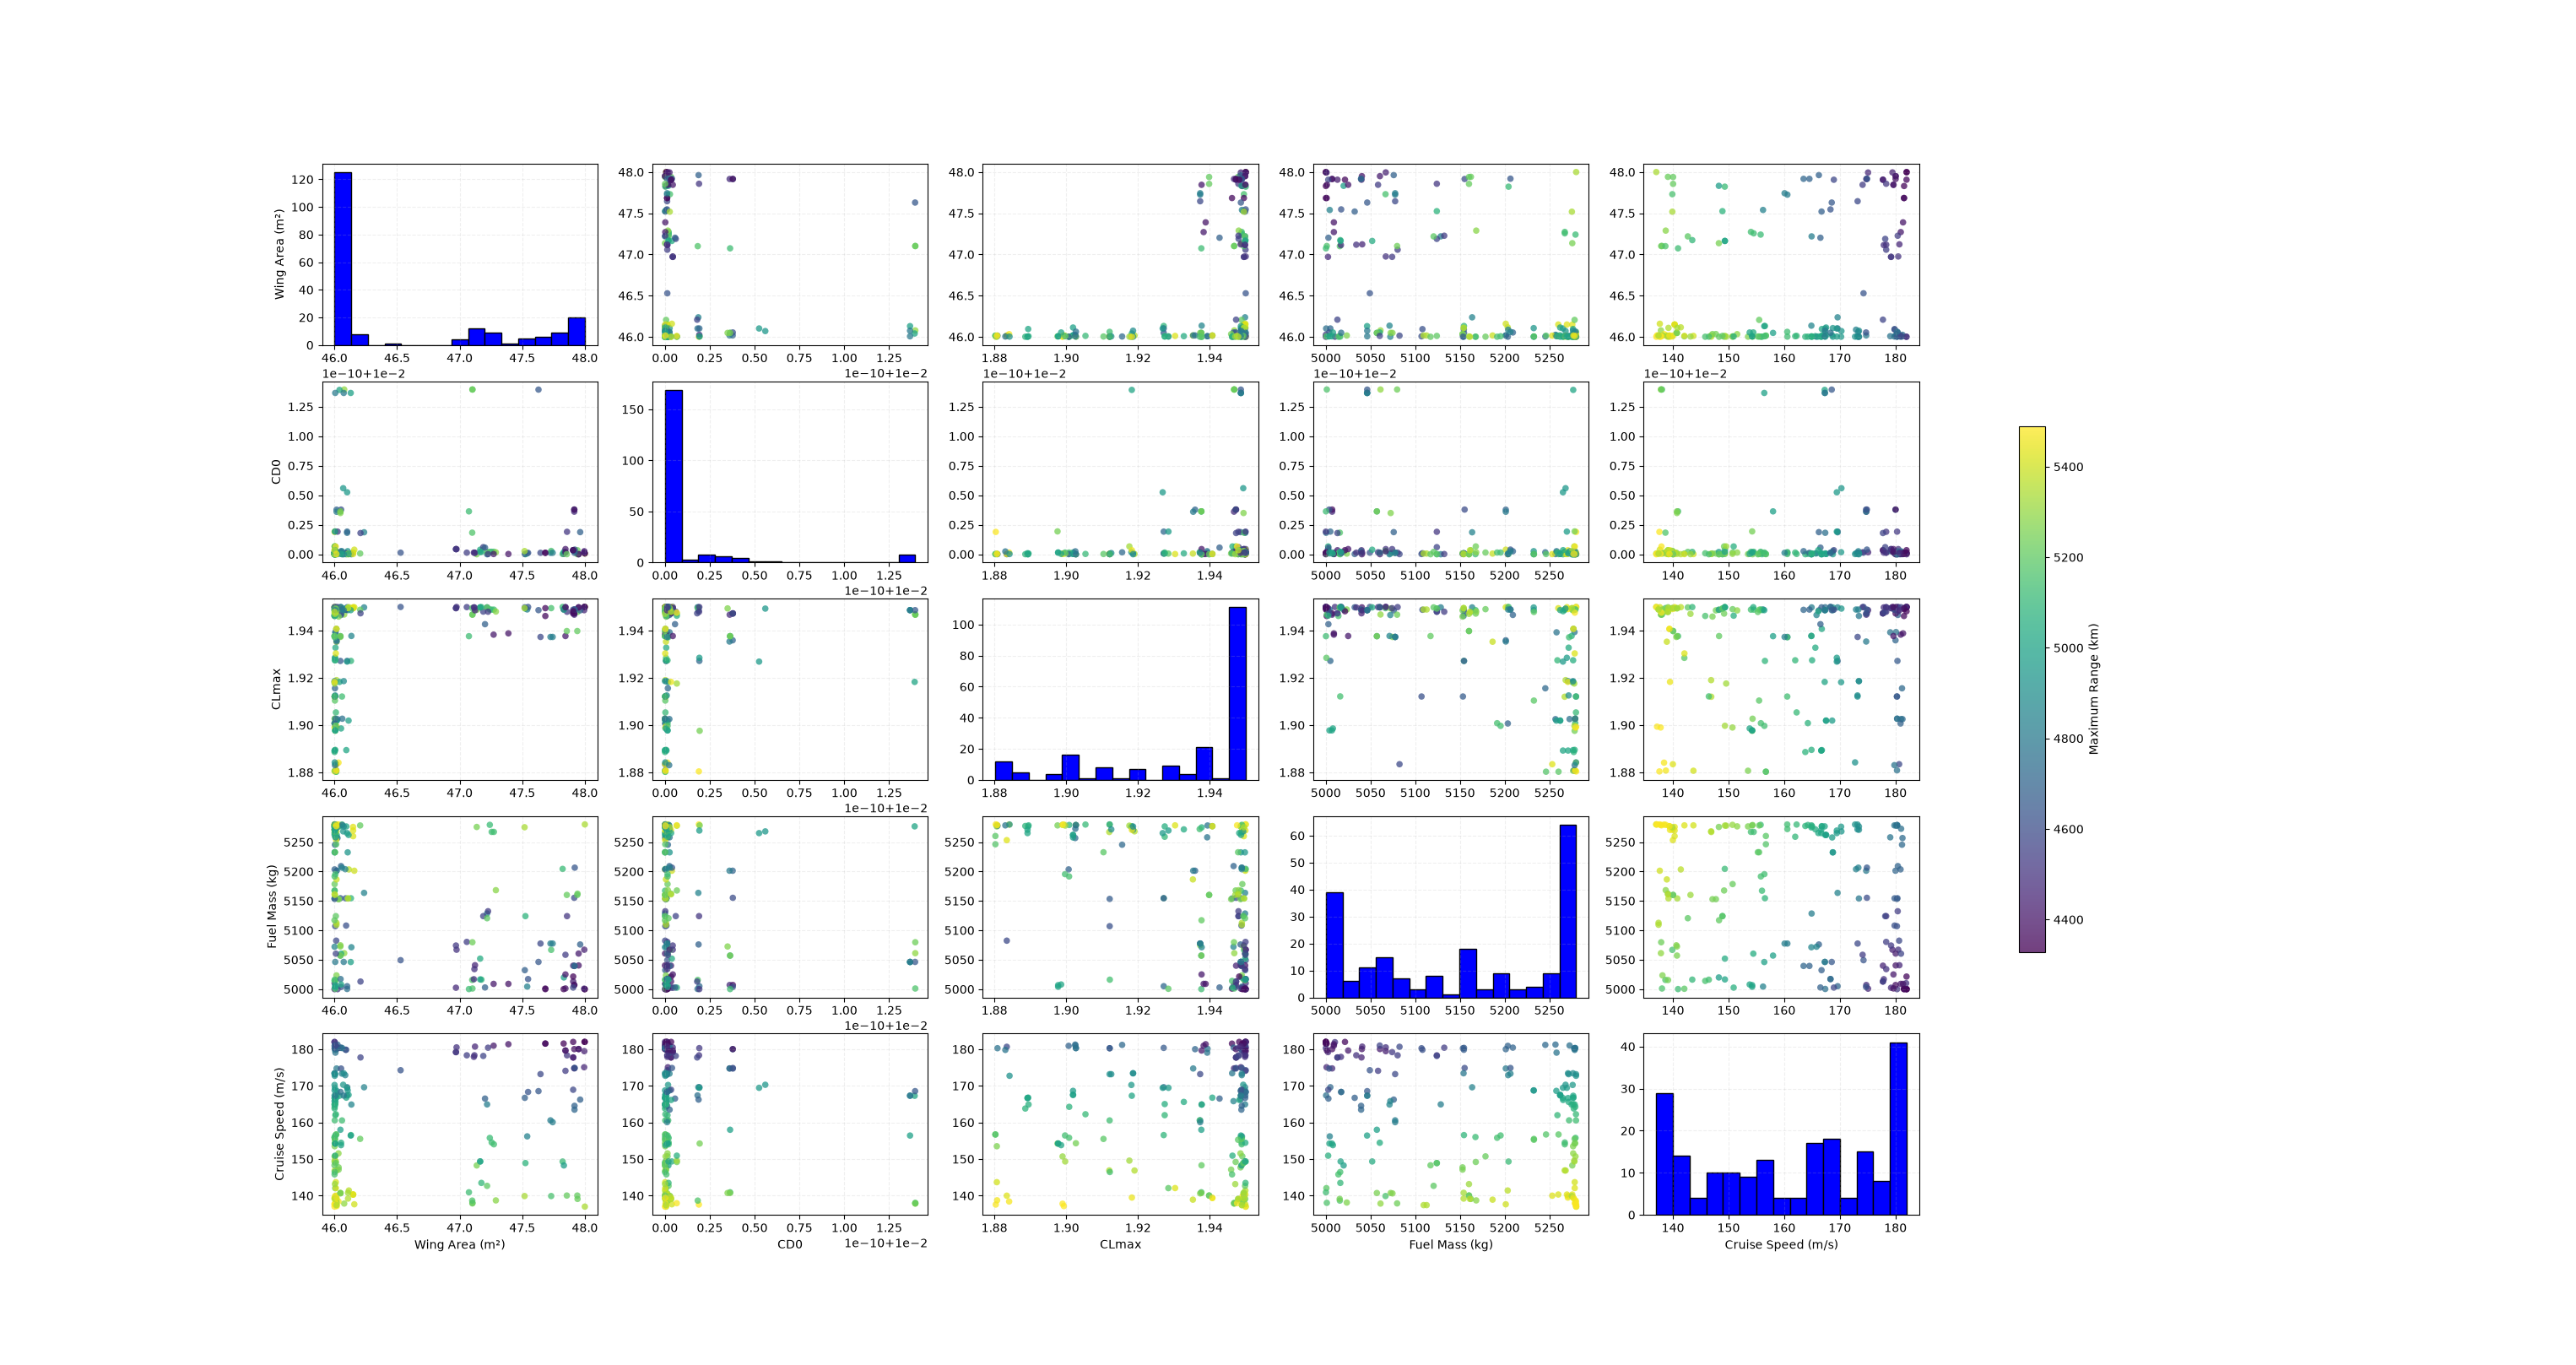
\includegraphics[width=\linewidth]{../UTIL/FIGS/DV-pareto-with-range.png}
        \caption[width=.7\linewidth]{Pareto-optimal design variables, with range visible}
        \label{fig:paretoDV}
\end{figure}

Should some DVs become preferred over others, a constraint based analysis would be more suitable, showing robust regions instead of a single value.
